%---------------------导言区---------------------------%
\documentclass[10pt,a4paper,twocolumn,twoside,UTF8]{ctexart}
\usepackage{geometry}
	\geometry{left=2cm,right=2cm,top=2.5cm,bottom=3cm}
\usepackage{xeCJK,amsmath,paralist,enumitem,booktabs,multirow,graphicx,subfig,setspace,listings}
	\setlength{\parindent}{2em}
	\lstset{language=Python}
\usepackage{titlesec}
	\newfontfamily\sectionef{Times New Roman}
	\setCJKfamilyfont{dsf}{Droid Sans Fallback}
 	\newcommand{\sectioncf}{\CJKfamily{dsf}}
  	\titleformat*{\section}{\large\bfseries\sectioncf\sectionef}
    \titleformat*{\subsection}{\normalsize\bfseries\sectioncf\sectionef}
\usepackage{fancyhdr}
\usepackage{layout}
\setlength\columnsep{0.8cm}
%%begin----------设置首页和正文不同的页眉页脚----------------%%
\usepackage{ifthen}
\newboolean{first}
\setboolean{first}{true}
\pagestyle{fancy}
	\fancypagestyle{maincontent}{
		\fancyhf{}  
		\fancyhead[EL, OR]{\thepage}
		\fancyhead[EC]{B6/B14 交流电桥测电感电容及Multisim电路仿真}
		\fancyhead[OC]{基\quad 础\quad 物\quad 理\quad 实\quad 验}
		\renewcommand\headrulewidth{0pt}
	}
	
	\usepackage{datetime}
	\fancypagestyle{firstpage}{
		\setboolean{first}{false}
		\fancyhf{}  
		\fancyhead[L]{\the\year 年\the\month 月}
		\fancyhead[R]{\shortmonthname[\the\month], \the\year}
		\fancyhead[C]{
		          \large{基\quad 础\quad 物\quad 理\quad 实\quad 验}\\
		          \normalsize{GENERAL PHYSICS LABORATORY}
		          }
	}
	
	\newcommand{\makefirstpageheadrule}{
	\makebox[0pt][s]{\rule[0.6\baselineskip]{\headwidth}{0.3pt}}
	\makebox[0pt][s]{\protect\hspace{-0.34em}\rule[0.75\baselineskip]{\headwidth}{0.3pt}}
	\protect\vspace{-20pt}
	}

	\newcommand{\makeheadrule}{
	\makebox[0pt][l]{\rule[1\baselineskip]{\headwidth}{0.3pt}}
	\protect\vspace{-20pt}
	}

	\renewcommand{\headrule}{
	\ifthenelse{\boolean{first}}{\makeheadrule}
	{\makefirstpageheadrule}
	}
%%end--------------设置首页和正文不同的页眉页脚-----------%%
%%begin-----------------参考文献-----------------------%%

\usepackage[colorlinks,linkcolor=blue,urlcolor=blue,citecolor=blue]{hyperref}
\usepackage[hyperref=true,backend=biber,bibstyle=gb7714-2015,citestyle=numeric-comp,sorting=none,backref=true]{biblatex}
\addbibresource{B6.bib}
%%end-------------------参考文献-----------------------%%

%%%%%%%%%%%%%%%%%%%%%%%%%%%%%%%%%%%%%%%%%%%%%%%%%%%%%%%%%%
%%%%%%%%%%%%%%%%%%%%%%%%%正文开始%%%%%%%%%%%%%%%%%%%%%%%%%%
%%%%%%%%%%%%%%%%%%%%%%%%%%%%%%%%%%%%%%%%%%%%%%%%%%%%%%%%%%

%%begin-------------------中文摘要-----------------------%%
\begin{document}
\title{\LARGE\textbf{B6/B14 交流电桥测电感电容及Multisim电路仿真} \footnotemark[1]}
\author{\large\textit{黄子维}$^{1}$\footnotemark[2]
\\ \normalsize{(1 \textit{中山大学 中山医学院,广东 广州 }510275)}}
\date{}

\twocolumn[
	\begin{@twocolumnfalse}
	\maketitle  
  	\renewcommand{\abstractname} {} 
	\begin{abstract}
	\vspace{-3em}
	{\bf 摘{} 要:}
	{\small 交流电桥是一种经典的实验电路。依据电桥平衡原理,可以利用交流电桥测量未知电路元件参数。
    这种测量方法简单便捷而精度高,在高精度测量,自动控制等领域有着广泛的应用。
    本实验中,我们利用电容电桥测量未知电容的电容、阻抗和损耗因数,用麦克斯威尔-维恩电桥测量未知电感的电感、阻抗和品质因数,并与数字电桥仪测量结果进行对比。
    同时我们还在$Multisim$电路仿真平台上进行了仿真实验,并与真实实验结果进行对比,探究影响本次实验结果的因素。
    实验发现,电容测量结果与数字电桥及仿真相差较大,后两者结果相近;而电感测量结果与仿真结果相近,数字电桥测量与前两者相差较大。
    本次实验的关键点是对交流电桥平衡状态调节的精细程度,而限制实验精度的最大因素是实验仪器的精密程度。}
	\par
	\textbf{关键词}:交流电桥,电容,电感,$Multisim$仿真实验
	\vspace{2em}
	\end{abstract}
	\end{@twocolumnfalse}
]
\renewcommand{\thefootnote}{\fnsymbol{footnote}}
\footnotetext[1]{由中山大学物理学院陆佑堂提供器材和指导。}
\footnotetext[2]{通信作者,\url{huangzw29@mail2.sysu.edu.cn}}
%%end-------------------中文摘要-----------------------%%

\thispagestyle{firstpage} %首页风格
\pagestyle{maincontent} %其他页风格

%%begin-------------------引言-----------------------%%
\section{引 \quad 言}
电桥是一种经典电路,利用电桥平衡原理,可用电桥测量未知电路元件参数。
交流电桥是工作在交流电下的电桥,可用于测量交流电路中各种电路元件参数,如电容、电感、阻抗等,
也可测量互感、磁性材料的磁导率等与电容、电感有关的其他物理量。
交流电桥在许多领域有着重要应用,Gearhart等人利用交流电桥构造了高灵敏度低温温度计\autocite{gearhartSimpleHighStability1975},
Jelinek等人利用交流电桥测量岩石磁化率及其各向异性\autocite{jelinekPrecisionBridgeSet1973}。
这些工作显示了交流电桥的广泛应用潜力。

经典交流电桥需要手动调节电桥平衡,步骤较为繁琐,这给元件快速测量和交流电桥应用推广带来阻碍。
Helbach等人在1983年提出了高精度自动数字交流电桥的实现方法\autocite{helbachHighPrecisionAutomaticDigital1983},
Holmberg等人在1995年提出了线性交流电桥的自动平衡方法\autocite{holmbergAutomaticBalancingLinear1995},
这些工作为数字交流电桥仪器提供了理论基础。本实验中,我们使用了数字交流电桥对元件进行测量,并与手动测量结果进行对比。

$Multisim$是美国国家仪器(NI)有限公司研制的电子线路仿真平台,具有强大的仿真实验功能,能够对模拟、数字、模拟/数字混合电路进行仿真。
我们在$Multisim 12.0$仿真平台上搭建交流电桥电路,进行仿真测量,并将仿真结果与真实实验进行对比。
同时我们还进行了RLC电路、非平衡直流电桥电路和的仿真实验,以掌握$Multisim$平台实验方法。

本实验目的是学习交流电桥原理,并运用交流电桥测量未知的电感、电容以及相关参数,探究影响实验结果的因素。

% \newpage %换栏
%%end-------------------引言-----------------------%%

%%begin-------------------正文-----------------------%%
\section{实验原理\autocite{shenJiChuWuLiShiYan2015}}

	\subsection{交流电桥及其平衡条件}
	交流电桥基本电路结构如图\ref{fig:illus-1}所示,$Z_1$、$Z_2$、$Z_3$、$Z_4$分别为四个桥臂的复阻抗。
		\begin{figure}[htbp]
			\centering
			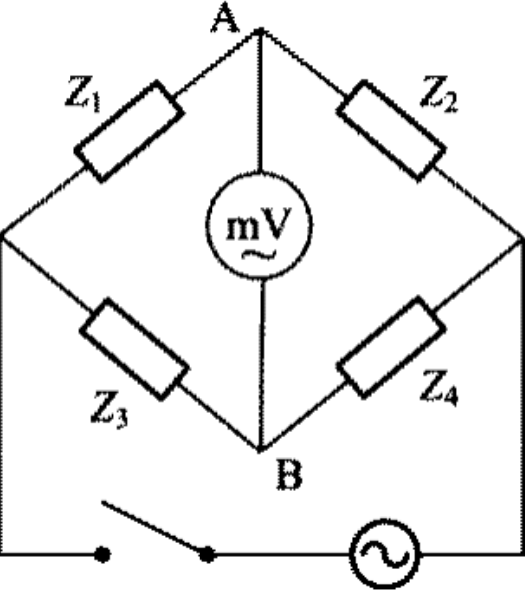
\includegraphics[width=0.25\textwidth]{attachments/illus-1.png}
			\caption{交流电桥基本结构}
			\label{fig:illus-1}
		\end{figure}

	调节各臂阻抗,使AB两点间的电位差为零,则电桥达到平衡,则有:
		\begin{align}
			\frac{Z_1}{Z_2} &= \frac{Z_3}{Z_4} \\
			\frac{|Z_1|e^{j\phi_1}}{|Z_2|e^{j\phi_2}} &= \frac{|Z_3|e^{j\phi_3}}{|Z_4|e^{j\phi_4}}
		\end{align}

	即:
		\begin{align}
			\frac{|Z_1|}{|Z_2|} &= \frac{|Z_3|}{|Z_4|} \\
			\phi_1-\phi_2 &= \phi_3-\phi_4
		\end{align}
	
	利用电桥平衡条件,可以确定未知电路元件的复阻抗,进而求出元件其余参数。

		\subsubsection{测量未知电容:电容电桥}
		电容电桥电路如图\ref{fig:illus-2}。$R_2$和$R_4$为纯电阻,
		$C_0$为标准电容,其损耗电阻$r_{C_0}$在低频时可近似为零。
		为与未知电容损耗电阻$r_C$相平衡,$C_0$串联了一个电阻$R_0$。
		\begin{figure}[htbp]
			\centering
			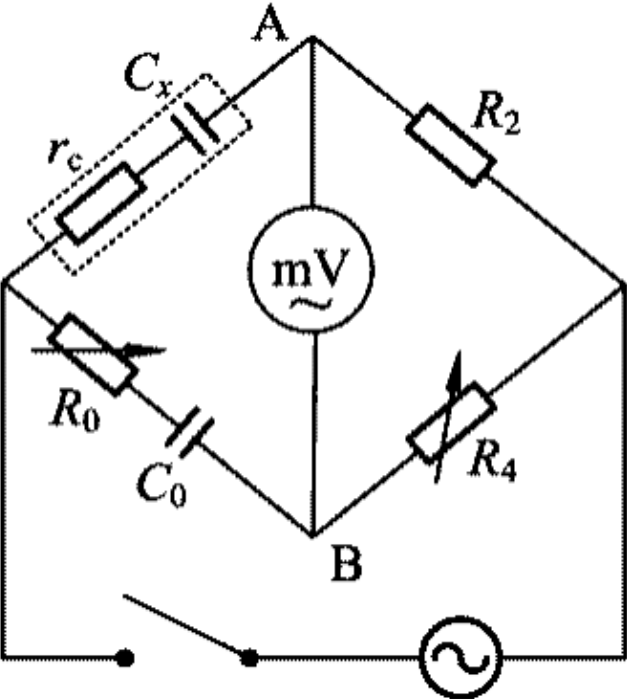
\includegraphics[width=0.25\textwidth]{attachments/illus-2.png}
			\caption{电容电桥}
			\label{fig:illus-2}
		\end{figure}

		根据电桥各臂配置,电桥平衡时有:
			\begin{gather}
				C_x = \frac{C_0R_4}{R_2} \label{eq:1.1} \\
				r_C = \frac{R_0R_2}{R_4} \label{eq:1.2} \\
				Z = \sqrt{(\frac{1}{\omega_0 C_x})^2+(r_C)^2} \label{eq:1.3} \\
				D = \omega_0r_CC_x = \omega_0R_0C_0 \label{eq:1.4}
			\end{gather}

		\subsubsection{测量未知电感:麦克思威尔-维恩电桥}
		电容电桥电路如图\ref{fig:illus-3}。$R_2$和$R_3$为纯电阻,
		$C_0$为标准电容,其损耗电阻$r_{C_0}$在低频时可近似为零。
		为与未知电感损耗电阻$r_L$相平衡,$C_0$串联了一个电阻$R_0$。
		\begin{figure}[htbp]
			\centering
			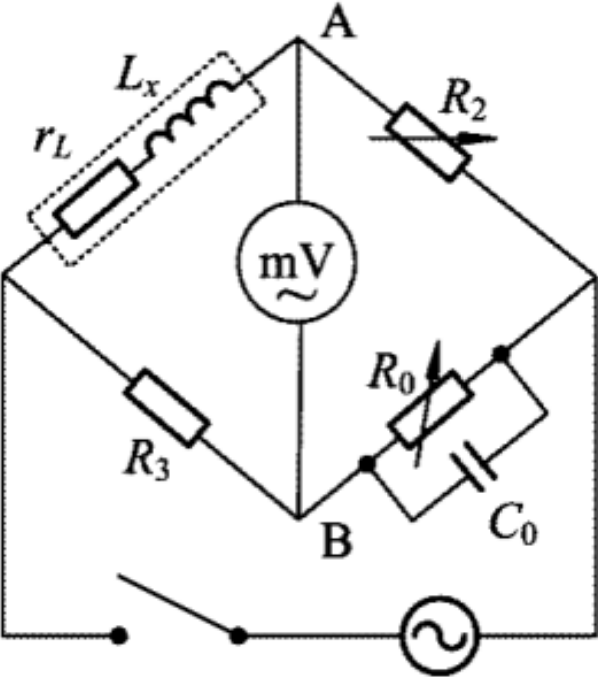
\includegraphics[width=0.25\textwidth]{attachments/illus-3.png}
			\caption{电感电桥}
			\label{fig:illus-3}
		\end{figure}

		根据电桥各臂配置,电桥平衡时有:
			\begin{gather}
				L_x = C_0R_2R_3 \label{eq:2.1} \\
				r_L = \frac{R_3R_2}{R_0} \label{eq:2.2} \\
				Z = \sqrt{(\omega_0 L_x)^2+(r_L)^2} \label{eq:2.3} \\
				D = \frac{\omega_0L_x}{r_L} = \omega_0R_0C_0 \label{eq:2.4}
			\end{gather}
	
	\subsection{其他两个仿真实验}
		\subsubsection{RLC电路仿真}
		RLC电路如图\ref{fig:illus-4}(a)。
		RLC电路总阻抗$Z$,电流$I$,电压电流相位差$\Delta\varphi$以及谐振频率$f_0$分别为:
		\begin{align}
			Z &= \sqrt{R^2+(\omega L-(\frac{1}{\omega C}))^2} \\
			I &= \frac{U}{\sqrt{R^2+(\omega L-(\frac{1}{\omega C}))}} \\
			\Delta \varphi &= -tan^{-1}(\frac{\omega L-(\frac{1}{\omega C})}{R}) \\
			f_0 &= \frac{1}{2\pi\sqrt{LC}}
		\end{align}

		根据以上参量可以画出RLC电路的幅频特性曲线(\ref{fig:illus-4}(b))和相频特性曲线\ref{fig:illus-4}(c)。
		\begin{figure}[htbp]
			\centering
			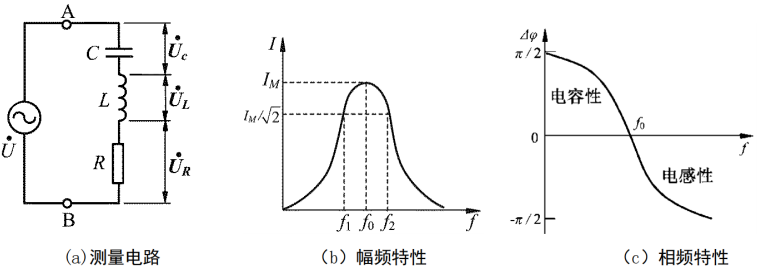
\includegraphics[width=0.4\textwidth]{attachments/illus-4.png}
			\caption{RLC电路的电路图,幅频特性和相频特性曲线}
			\label{fig:illus-4}
		\end{figure}

		分别将RLC电路中的电容和电感短路,即可得到RL电路及RC电路,依照相似的原理也可分别画出幅频曲线和相频曲线。

		\subsubsection{非平衡直流电桥}
		非平衡直流电桥电路图如图\ref{fig:illus-5}。电桥不平衡时,万用表显示AB两点间的电压:
		\begin{equation}
			\Delta U = \frac{R_1R_4-R_3R_2}{(R_1+R_2)(R_3+R_4)}U \label{eq:3}
		\end{equation}

		改变两滑动变阻器的阻值可调节AB两点间的电势差。当AB间的电压0时电桥平衡,此时各电阻之间应满足的关系为:
		\begin{equation}
			R_1R_4 = R_3R_2
		\end{equation}
		
		\begin{figure}[htbp]
			\centering
			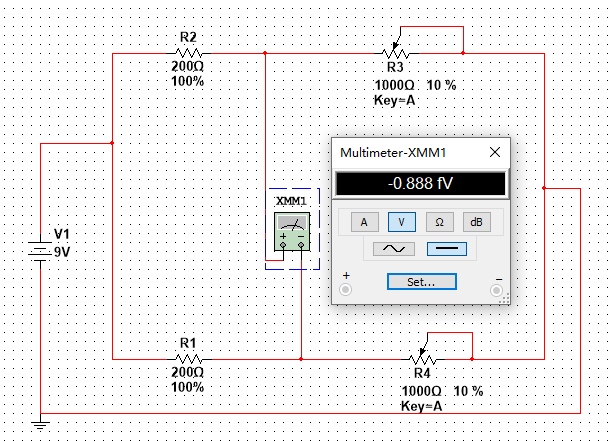
\includegraphics[width=0.4\textwidth]{attachments/illus-5.png}
			\caption{非平衡直流电桥}
			\label{fig:illus-5}
		\end{figure}


\section{实验仪器和平台}
	\paragraph{A. NI-VisualBench 一体化仪器(VB-8012)}
	本仪器具有函数信号发生器、示波器、数字万用表、直流稳压电源、逻辑分析仪等功能。
	连接测控计算机后,可以使用一体化仪器同时输出函数信号并测量电压。
	\paragraph{B. 数字自动电桥(TH2811D)}
	成品数字电桥内置交流电桥电路,基本原理与交流电桥相同,可以自动测量电容、电感等电路元件。
	\paragraph{C. 电路仿真平台(Multisim 12.0)}
	$Multisim$是美国国家仪器(NI)有限公司研制的电子线路仿真平台,具有强大的仿真实验功能,能够对模拟、数字、模拟/数字混合电路进行仿真。

\section{实验步骤}
	\subsection{利用交流电桥测量电容和电感}
	\begin{enumerate}[label=\arabic*.]
		\item 依照图\ref{fig:illus-2}连接电容电桥,依照图\ref{fig:illus-3}连接电感电桥。
		\item 使用$NI-VisualBench$一体化仪器函数发生功能作为信号输入,调节频率为$10kHZ$,电压幅值为$5V$,直流偏移为$0V$。
	 	\item 使用$NI-VisualBench$一体化仪器万用表功能,监测电桥AB点间交流电压。
	 	\item 调节电阻箱使电桥平衡状态,多次重复测量,记录各电阻箱的数值。
	 	\item 交叉换臂,调节电阻箱使电桥平衡状态,多次重复测量,记录各电阻箱的数值。
	 	\item 根据实验数据,分别计算待测电容、损耗电阻和损耗因数以及待测电感、损耗电阻和品质因数,并分析误差。
	 	\item 使用自动数字交流电桥测量待测电容和电感,将自动测量结果与手动调节实验结果进行对比。
	\end{enumerate}

	\subsection{Multisim平台仿真实验}
		\subsubsection{交流电桥仿真实验}
		在Multisim平台上搭建相同的交流电桥电路,调节各滑动变阻器使两桥臂间仿真万用表示数接近0,则电桥平衡。
		记录各电阻阻值,计算待测电容和电感参数,并与真实实验结果进行对比。
		\subsubsection{RLC电路仿真}
		在Multisim平台上搭建RLC电路,并运行仿真自动扫描,扫描频率范围为$0Hz \sim 10MHz$。
		利用仿真示波器,导出RLC电路的幅频特性曲线和相频特性曲线,并与实际 RLC 电路的幅频特性曲线和相频特性曲线对比分析。

		分别将电容和电感短路,得到RL电路或RC电路。采用相同的办法进行扫描,
		同样可以得到它们的幅频特性曲线和相频特性曲线,并与实际RL或RC电路的幅频特性曲线和相频特性曲线对比分析。
		\subsubsection{非平衡直流电桥仿真}
		设置$R_3$和$R_4$的初始值为$1000\Omega$,同步反向改变$R_3$和$R_4$的阻值$\Delta R$,
		使直流电桥两桥臂间电压表示数为$40,30,20,10,0mV$,记录两电阻阻值,探究电压变化$\Delta U$与$\Delta R$的关系。

	\subsection{黑箱电路分析实验}
	利用万用表和数字自动电桥,测量四端黑箱电路每两接线柱之间的电容、电阻、电感,根据测量结果分析黑箱中的电路。

\section{实验结果}
	\subsection{利用交流电桥测量电容和电感}
		\subsubsection{测量电容}
		实验原始数据如表\ref{tab:1.1}。实验中$C_0=0.47 \mu F$,$R_2 = 510 \Omega$。
			\begin{table}[htbp]
				\centering
					\begin{tabular}{ccc}
						\toprule
						$R_0 / \Omega$	&$R_4 / \Omega$	&$U /mV$ \\
						\midrule
						11.0	&132.0	&2.725	\\
						11.2	&132.2	&1.426	\\
						11.3	&132.3	&1.318	\\
						11.3	&132.3	&1.363	\\
						11.3	&132.3	&1.352	\\
						\midrule
						换臂 & & \\
						\midrule
						11.3	&133.0	&2.719	\\
						11.4	&133.0	&2.120	\\
						11.3	&133.0	&2.170	\\
						11.1	&133.0	&2.721	\\
						11.3	&133.0	&2.347	\\	
						\bottomrule
					\end{tabular}
					\caption{\textbf{电容电桥可调电阻阻值}}
					\label{tab:1.1}
			\end{table}

		由式\ref{eq:1.1},式\ref{eq:1.2},式\ref{eq:1.3}和式\ref{eq:1.4},
		代入$R_0$和$R_4$计算电容,损耗电阻,阻抗和损耗因数得
			\begin{gather}
				C_x = \frac{C_0R_4}{R_2} = 122 \pm 1 nF  \\
				r_C = \frac{R_0R_2}{R_4} = 43.3 \pm 0.5 \Omega \\
				Z = \sqrt{(\frac{1}{\omega_0 C_x})^2+(r_C)^2} = 137.2 \pm 0.5 \Omega \\
				D = \omega_0r_CC_x = \omega_0R_0C_0 =  0.33 \pm 0.004 
			\end{gather}

		\subsubsection{测量电感}
		实验原始数据如表\ref{tab:1.1}。实验中$C_0=0.47 \mu F$,$R_3 = 510 \Omega$。
			\begin{table}[htbp]
				\centering
					\begin{tabular}{ccc}
						\toprule
						$R_0 / \Omega$	&$R_2 / \Omega$	&$U /mV$ \\
						\midrule
						420.0	&84.7	&0.929	\\
						420.1	&84.7	&1.015	\\
						420.0	&84.8	&0.945	\\
						419.9	&84.8	&0.915	\\
						419.9	&84.7	&1.030	\\
						\midrule
						换臂 & & \\
						\midrule
						420.0	&80.2	&2.962	\\
						420.0	&80.1	&2.742	\\
						420.0	&80.0	&2.919	\\
						419.9	&80.1	&2.877	\\
						419.8	&80.1	&3.235	\\	
						\bottomrule
					\end{tabular}
					\caption{\textbf{电感电桥可调电阻阻值}}
					\label{tab:1.2}
			\end{table}

		由式\ref{eq:2.1},式\ref{eq:2.2},式\ref{eq:2.3}和式\ref{eq:2.4},
		代入$R_0$和$R_2$计算电感,损耗电阻,阻抗和品质因数得
			\begin{gather}
				L_x = C_0R_2R_3 = 19.8 \pm 0.5 mH\\
				r_L = \frac{R_3R_2}{R_0} = 100 \pm 3 \Omega \\
				Z = \sqrt{(\omega_0 L_x)^2+(r_L)^2} = 1245 \pm 37 \Omega \\
				D = \frac{\omega_0L_x}{r_L} = \omega_0R_0C_0 = 12.4 \pm 0.003
			\end{gather}

		\subsubsection{自动数字电桥验证测量结果}
		使用自动数字电桥测量待测电容和电感,结果如表\ref{tab:2}
		\begin{table}[htbp]
			\centering
				\begin{tabular}{cccc}
					\toprule
					电容	&	&电感	& \\
					\midrule
					$C_x$	&97.526$nF$	&$L_x$	&19.892$mH$	\\
					$r_C$	&52.50$\Omega$	&$r_L$	&133.87$\Omega$	\\
					$Z_C$	&171.43$\Omega$	&$Z_L$	&1257.0$\Omega$	\\
					$D$		&0.3221			&$Q$	&9.3062	\\
					\bottomrule
				\end{tabular}
				\caption{\textbf{自动数字电桥测量结果}}
				\label{tab:2}
		\end{table}

	\subsection{Multisim平台仿真实验}
		\subsubsection{交流电桥仿真实验}
			\paragraph{A. 电容电桥仿真}~
			\newline 
			\indent
			实验结果如图\ref{fig:1.1}。
			\begin{figure}[htbp]
				\centering
				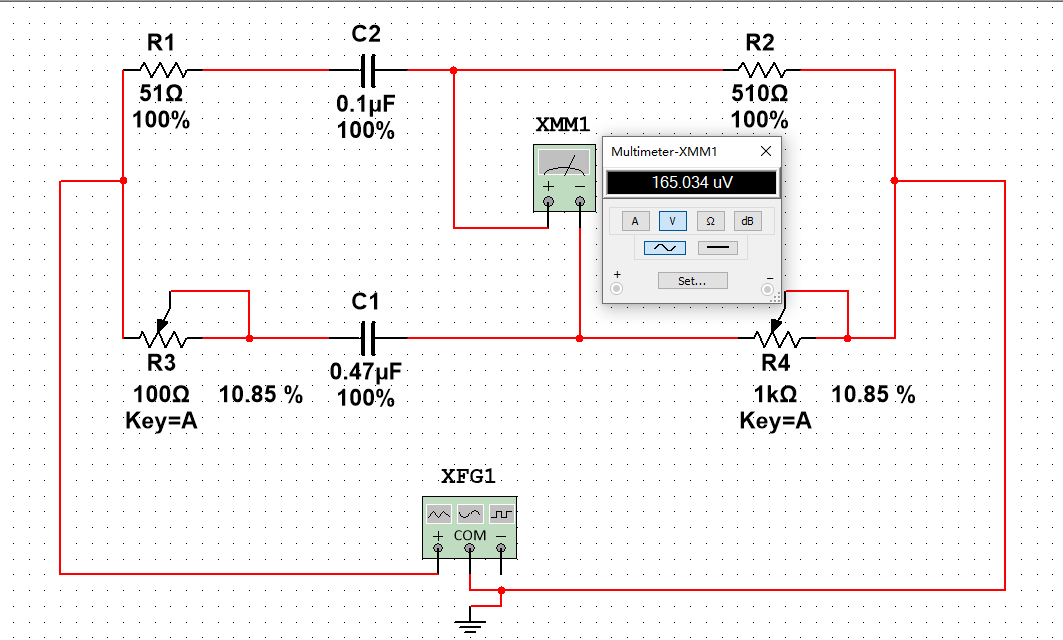
\includegraphics[width=0.5\textwidth]{attachments/fig.1.1.png}
				\caption{电容电桥}
				\label{fig:1.1}
			\end{figure}	
			由式\ref{eq:1.1},式\ref{eq:1.2},式\ref{eq:1.3}和式\ref{eq:1.4},
			代入$R_0 = 10.85 \Omega$和$R_4 = 108.5 \Omega$计算电容,损耗电阻,阻抗和损耗因数得
				\begin{gather}
					C_x = \frac{C_0R_4}{R_2} = 100.00 nF  \\
					r_C = \frac{R_0R_2}{R_4} = 51.00 \Omega \\
					Z = \sqrt{(\frac{1}{\omega_0 C_x})^2+(r_C)^2} = 167.1 \Omega \\
					D = \omega_0r_CC_x = \omega_0R_0C_0 =  0.32 
				\end{gather}

			\paragraph{B. 电感电桥仿真}~
			\newline 
			\indent
			实验结果如图\ref{fig:1.2}。
			\begin{figure}[htbp]
				\centering
				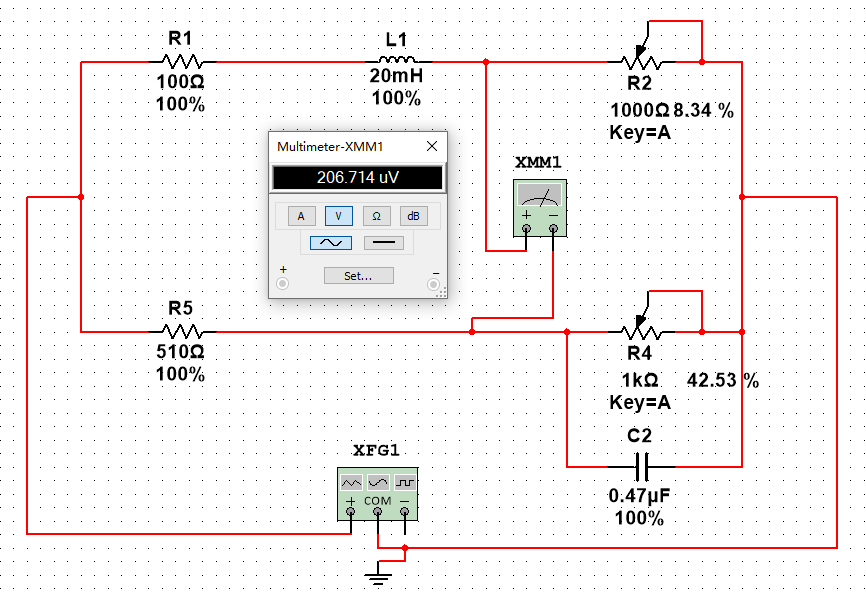
\includegraphics[width=0.5\textwidth]{attachments/fig.1.2.png}
				\caption{电感电桥}
				\label{fig:1.2}
			\end{figure}
			
			由式\ref{eq:2.1},式\ref{eq:2.2},式\ref{eq:2.3}和式\ref{eq:2.4},
			代入$R_0 = 83.4 \Omega $和$R_2 = 425.3 \Omega $计算电感,损耗电阻,阻抗和品质因数得
				\begin{gather}
					L_x = C_0R_2R_3 = 19.991 mH\\
					r_L = \frac{R_3R_2}{R_0} = 100.01 \Omega \\
					Z = \sqrt{(\omega_0 L_x)^2+(r_L)^2} = 1260.0 \Omega \\
					D = \frac{\omega_0L_x}{r_L} = \omega_0R_0C_0 = 12.6
				\end{gather}
		\subsubsection{RLC电路仿真实验}
			\paragraph{A. RLC电路}~
			\newline 
			\indent
			RLC电路仿真幅频曲线和相频曲线如图\ref{fig:2.1},对比B5实验结果,发现仿真与真实实验吻合。
			\begin{figure}[htbp]
				\centering
				\subfloat[RLC仿真实验结果]{\label{fig:2.1}
				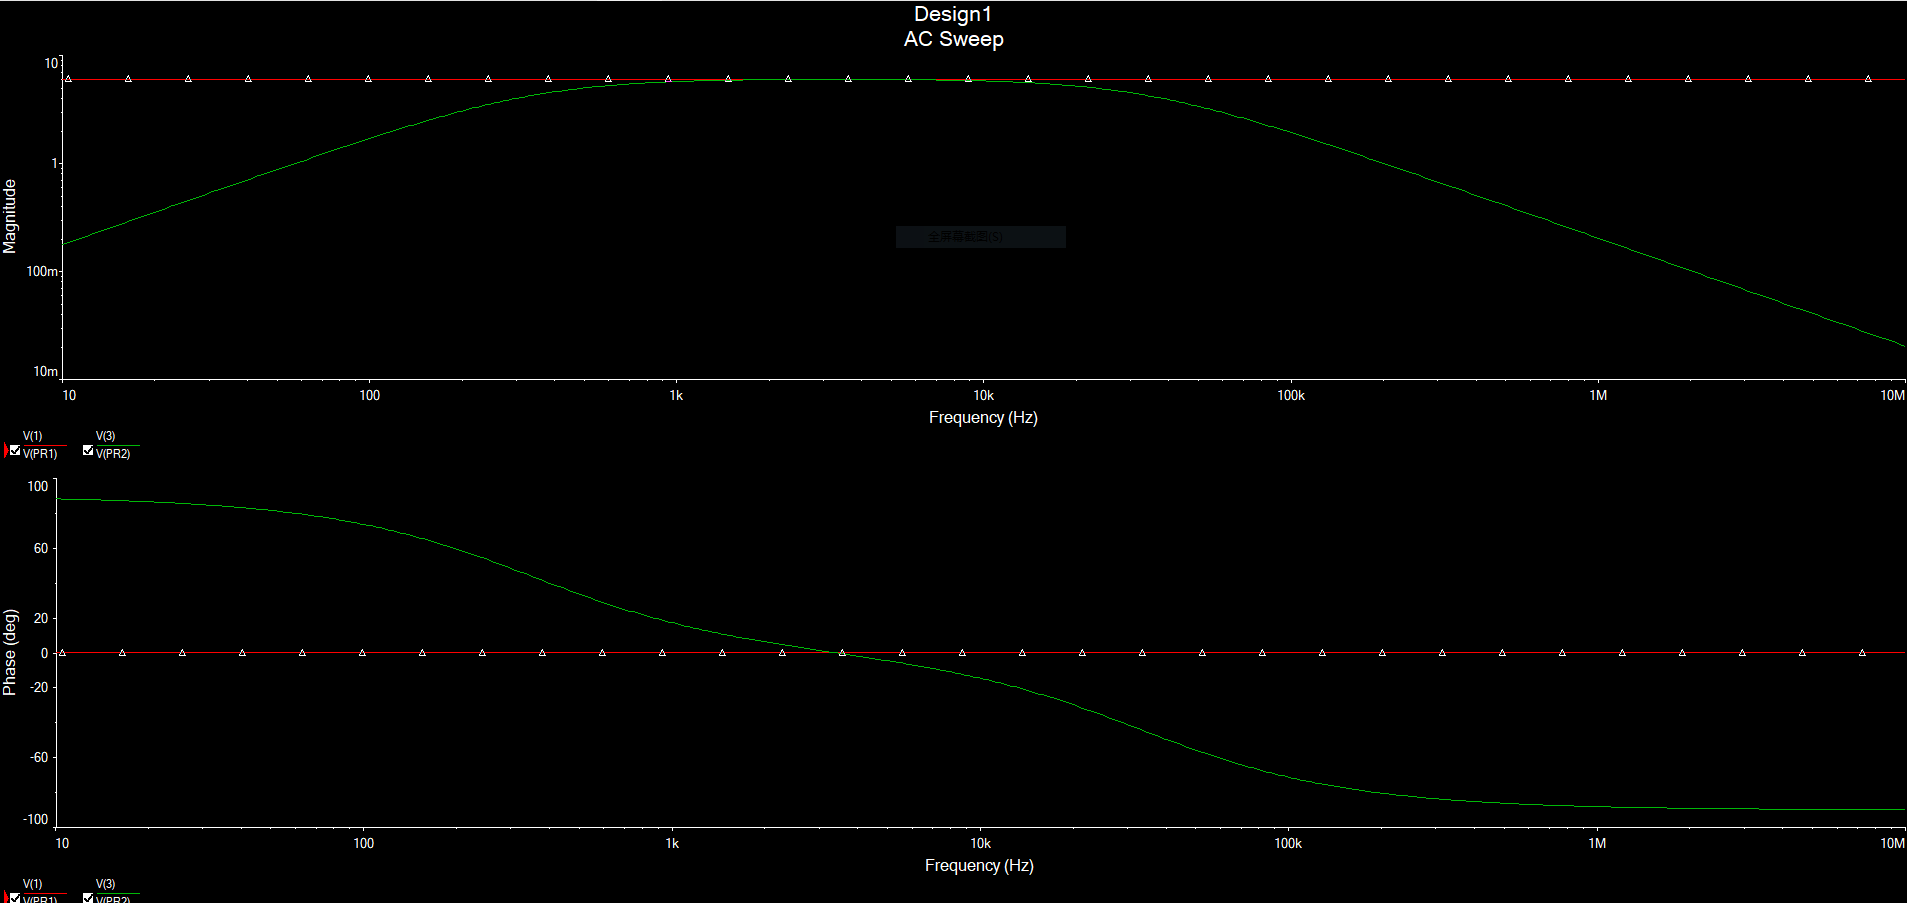
\includegraphics[width=0.3\textwidth]{attachments/fig.2.1.png}
				}
				
				\subfloat[实验幅频曲线]{\label{fig:2.1.1}
				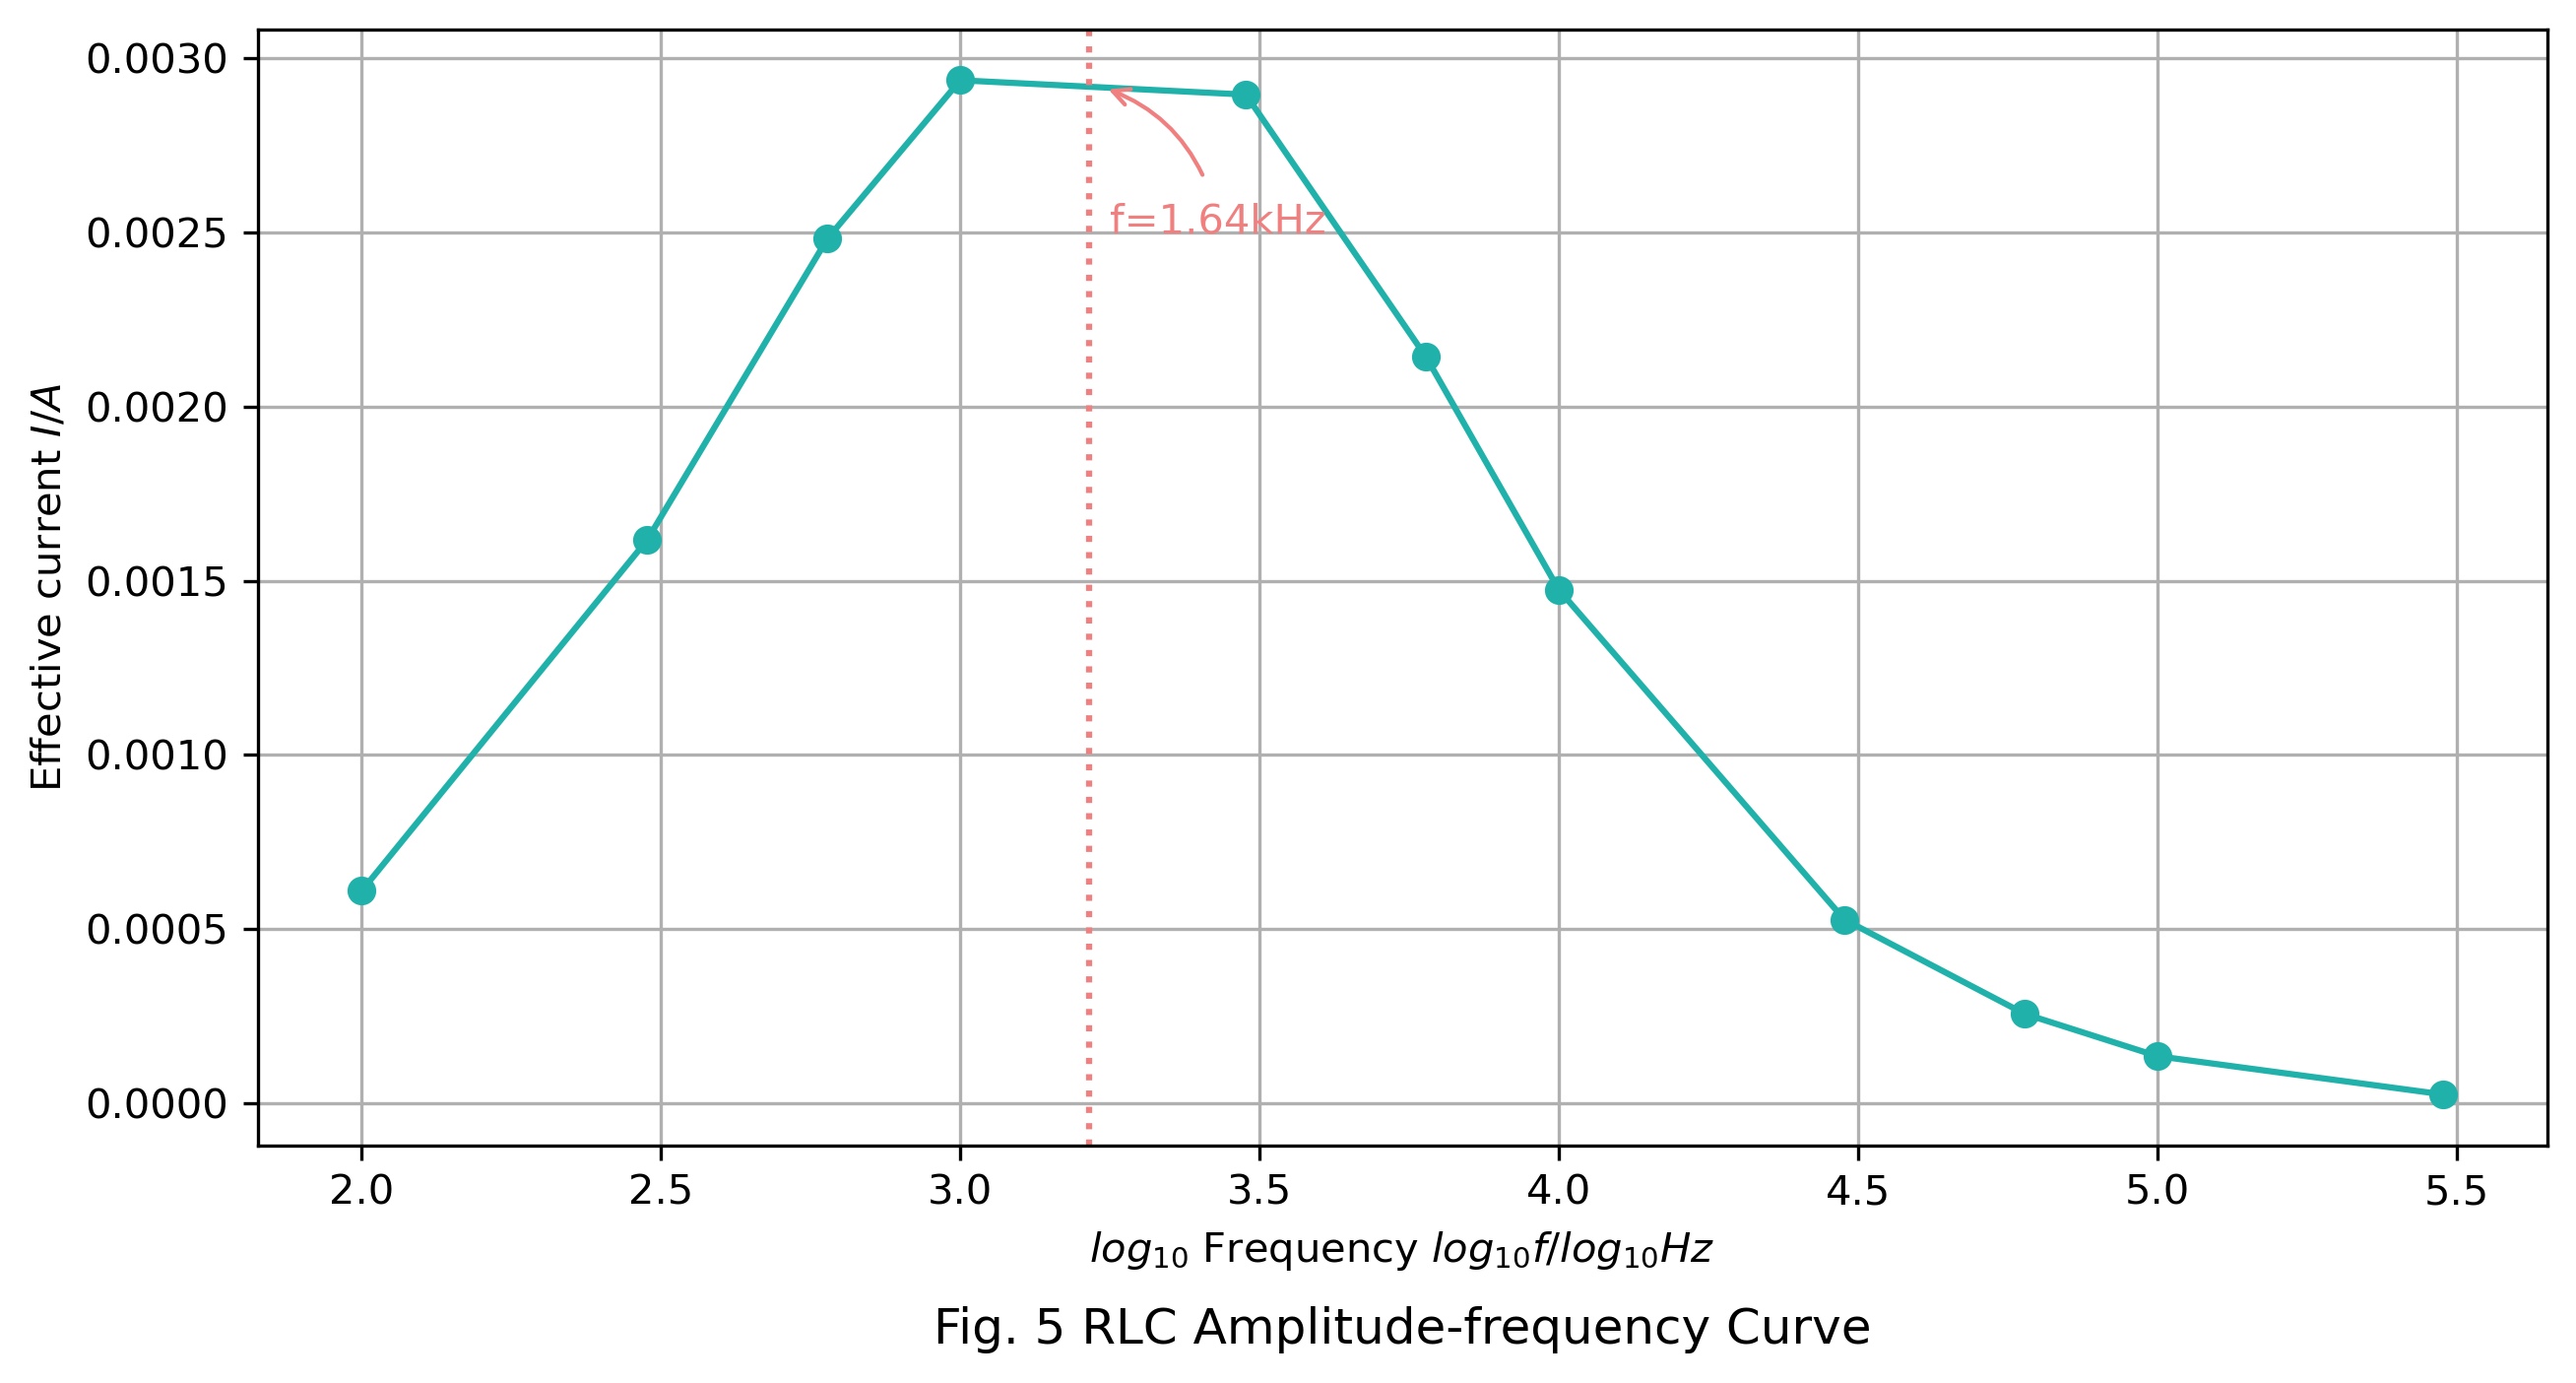
\includegraphics[width=0.23\textwidth]{attachments/fig.2.1.1.png}
				}
				\subfloat[实验相频曲线]{\label{fig:2.1.2}
				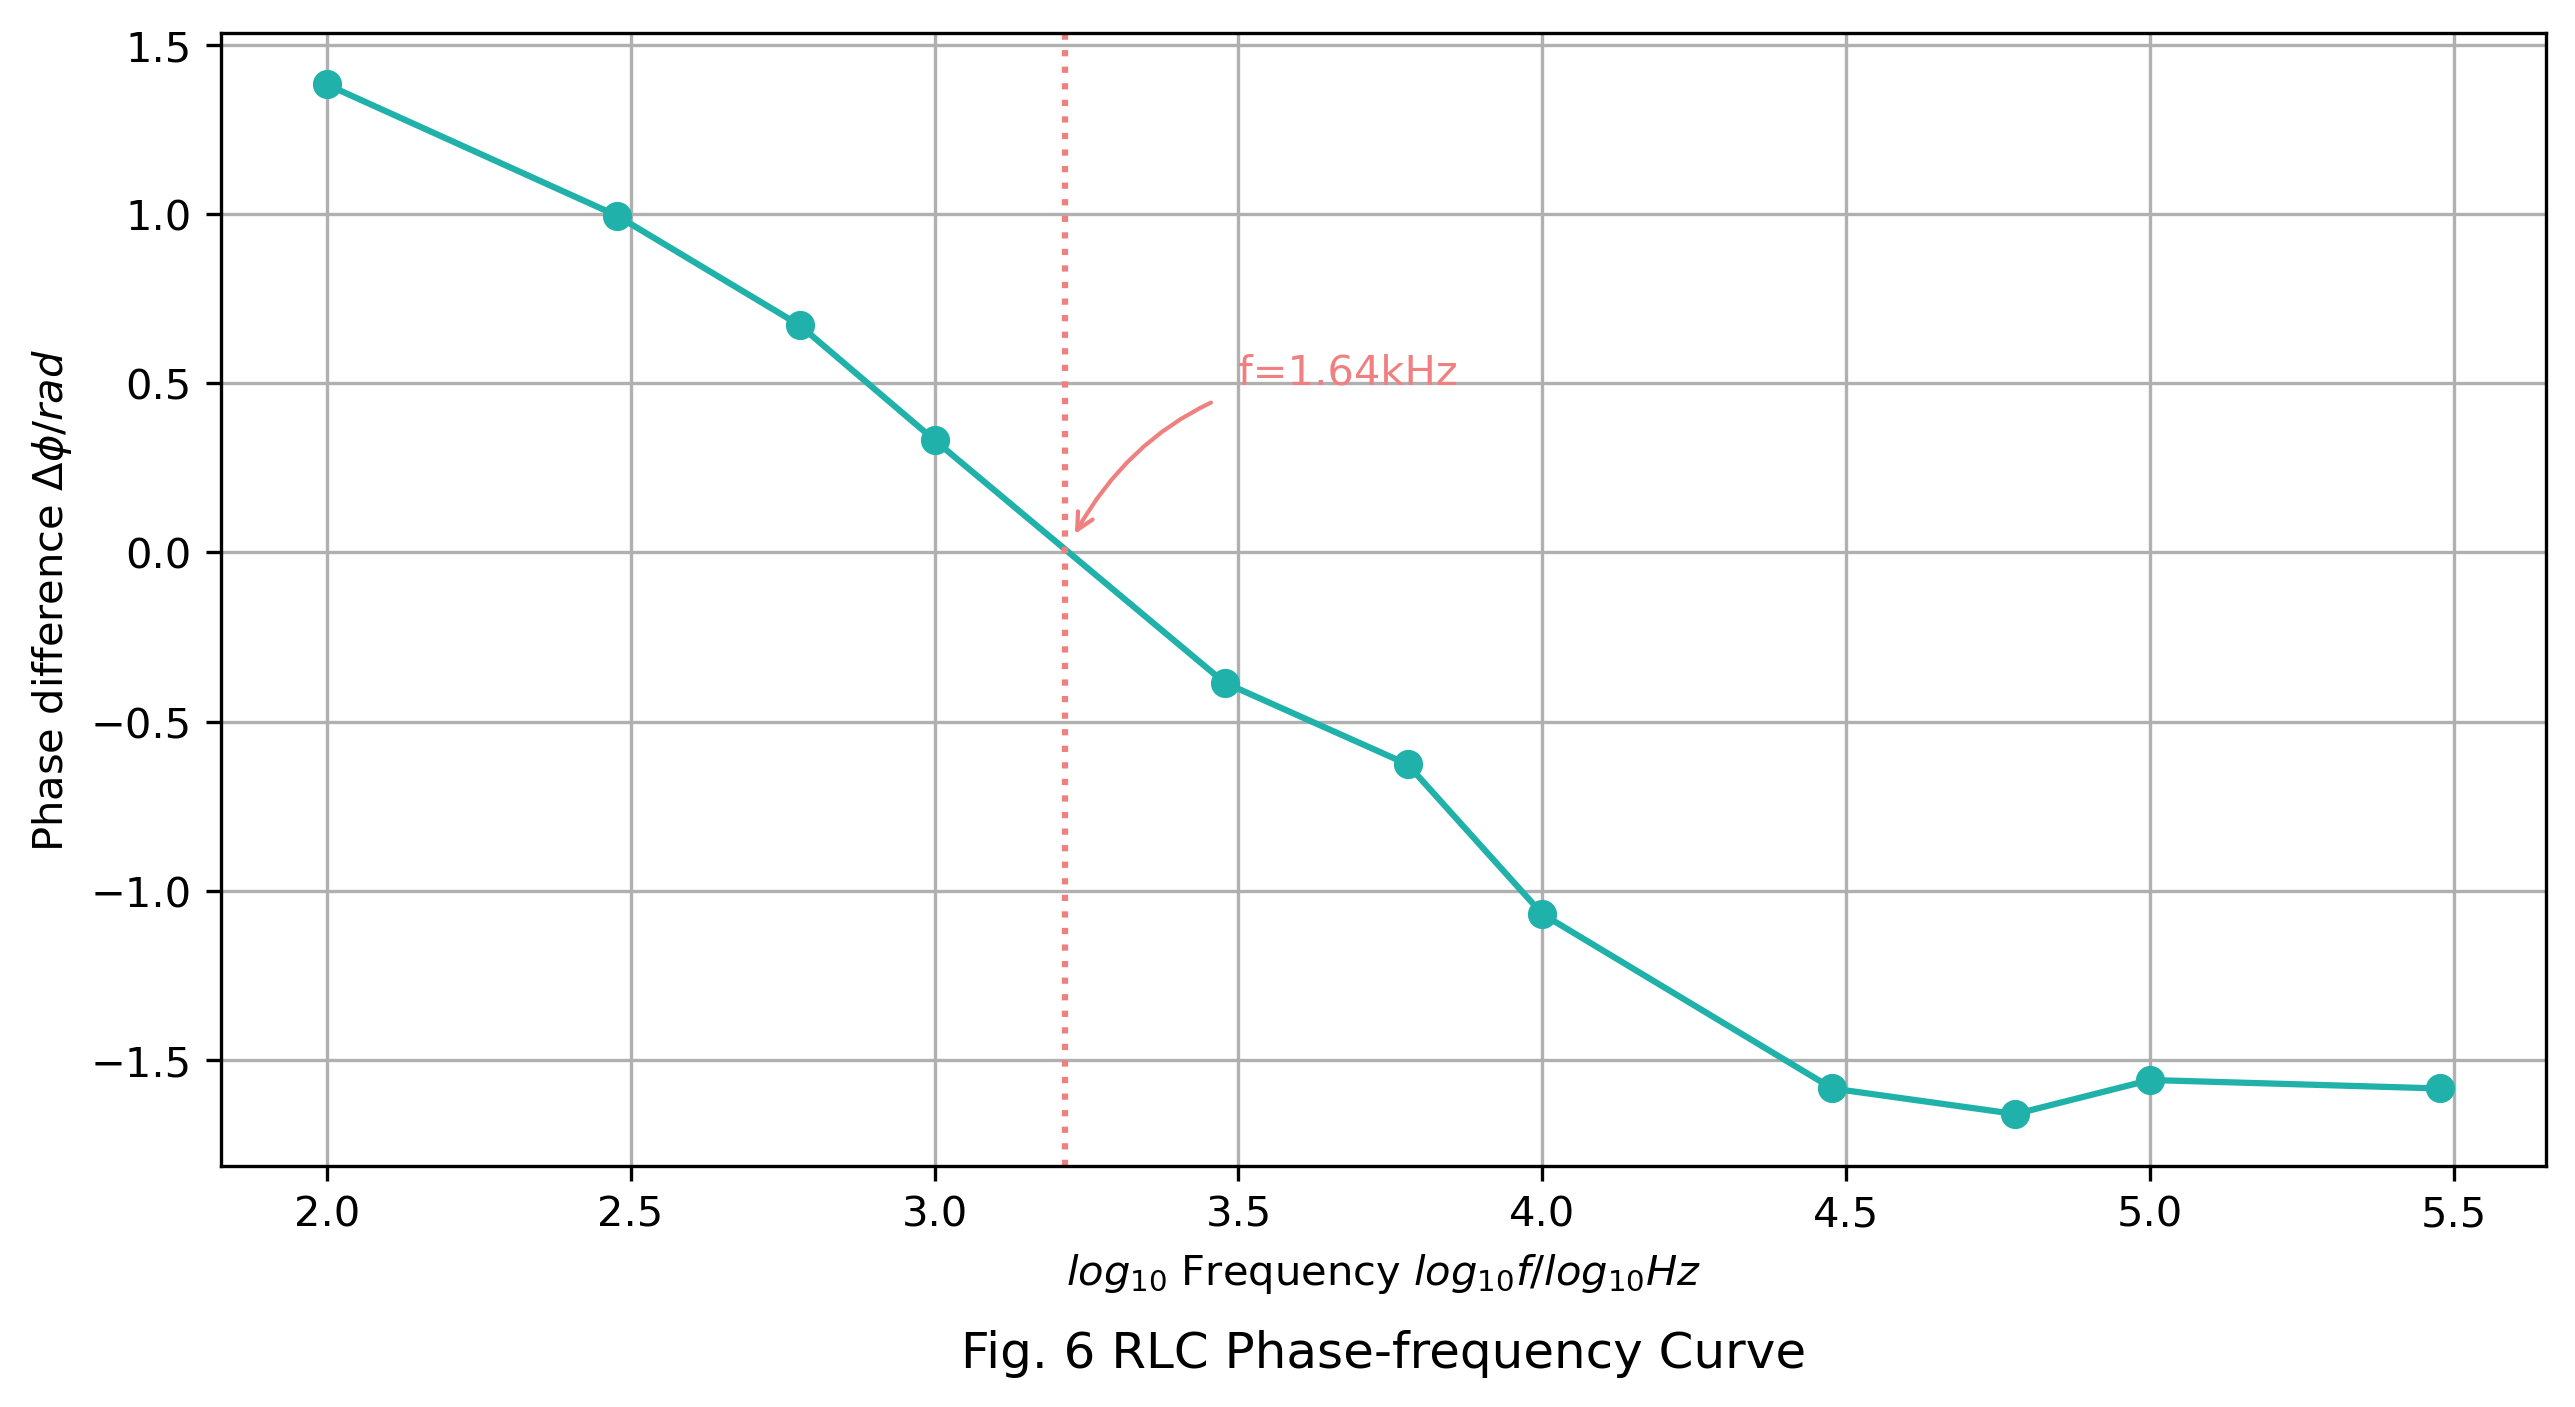
\includegraphics[width=0.23\textwidth]{attachments/fig.2.1.2.png}
				}
				\caption{RLC电路}
			\end{figure}

			\paragraph{B. RC电路}~
			\newline 
			\indent
			RC电路仿真幅频曲线和相频曲线如图\ref{fig:2.2},对比B5实验结果,发现仿真与真实实验吻合。
			\begin{figure}[htbp]
				\centering
				\subfloat[RC仿真实验结果]{\label{fig:2.2}
				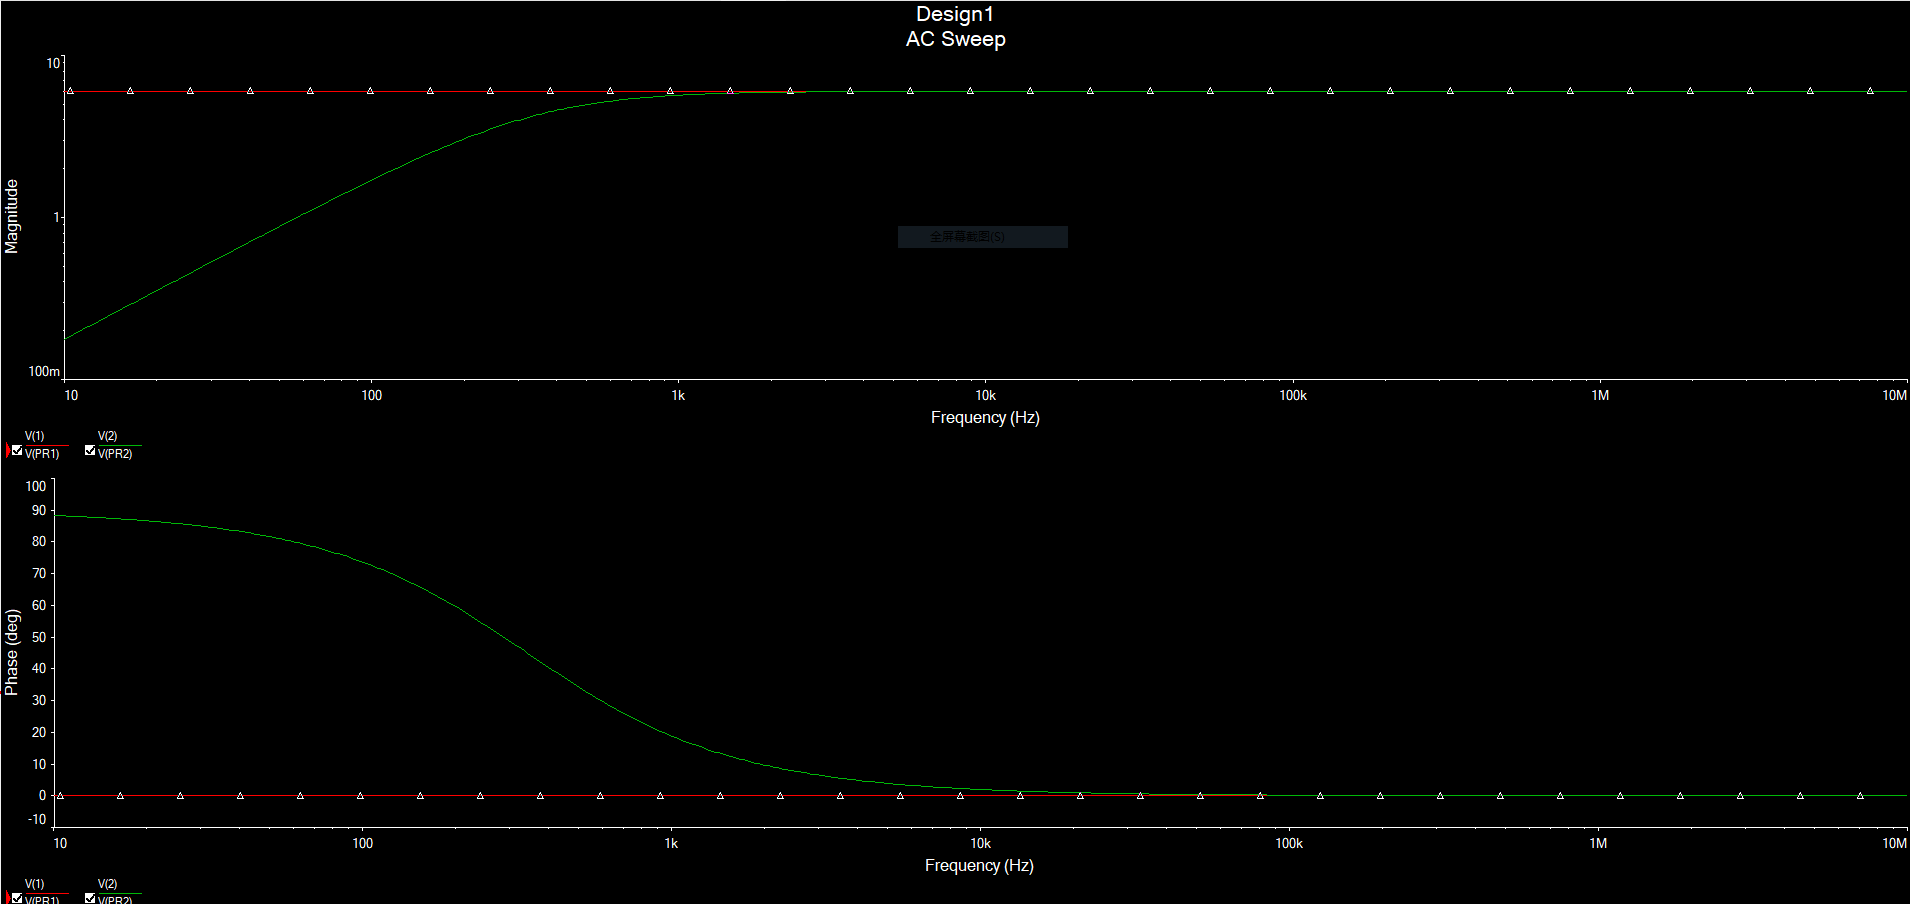
\includegraphics[width=0.3\textwidth]{attachments/fig.2.2.png}
				}	
				
				\subfloat[实验幅频曲线]{\label{fig:2.2.1}
				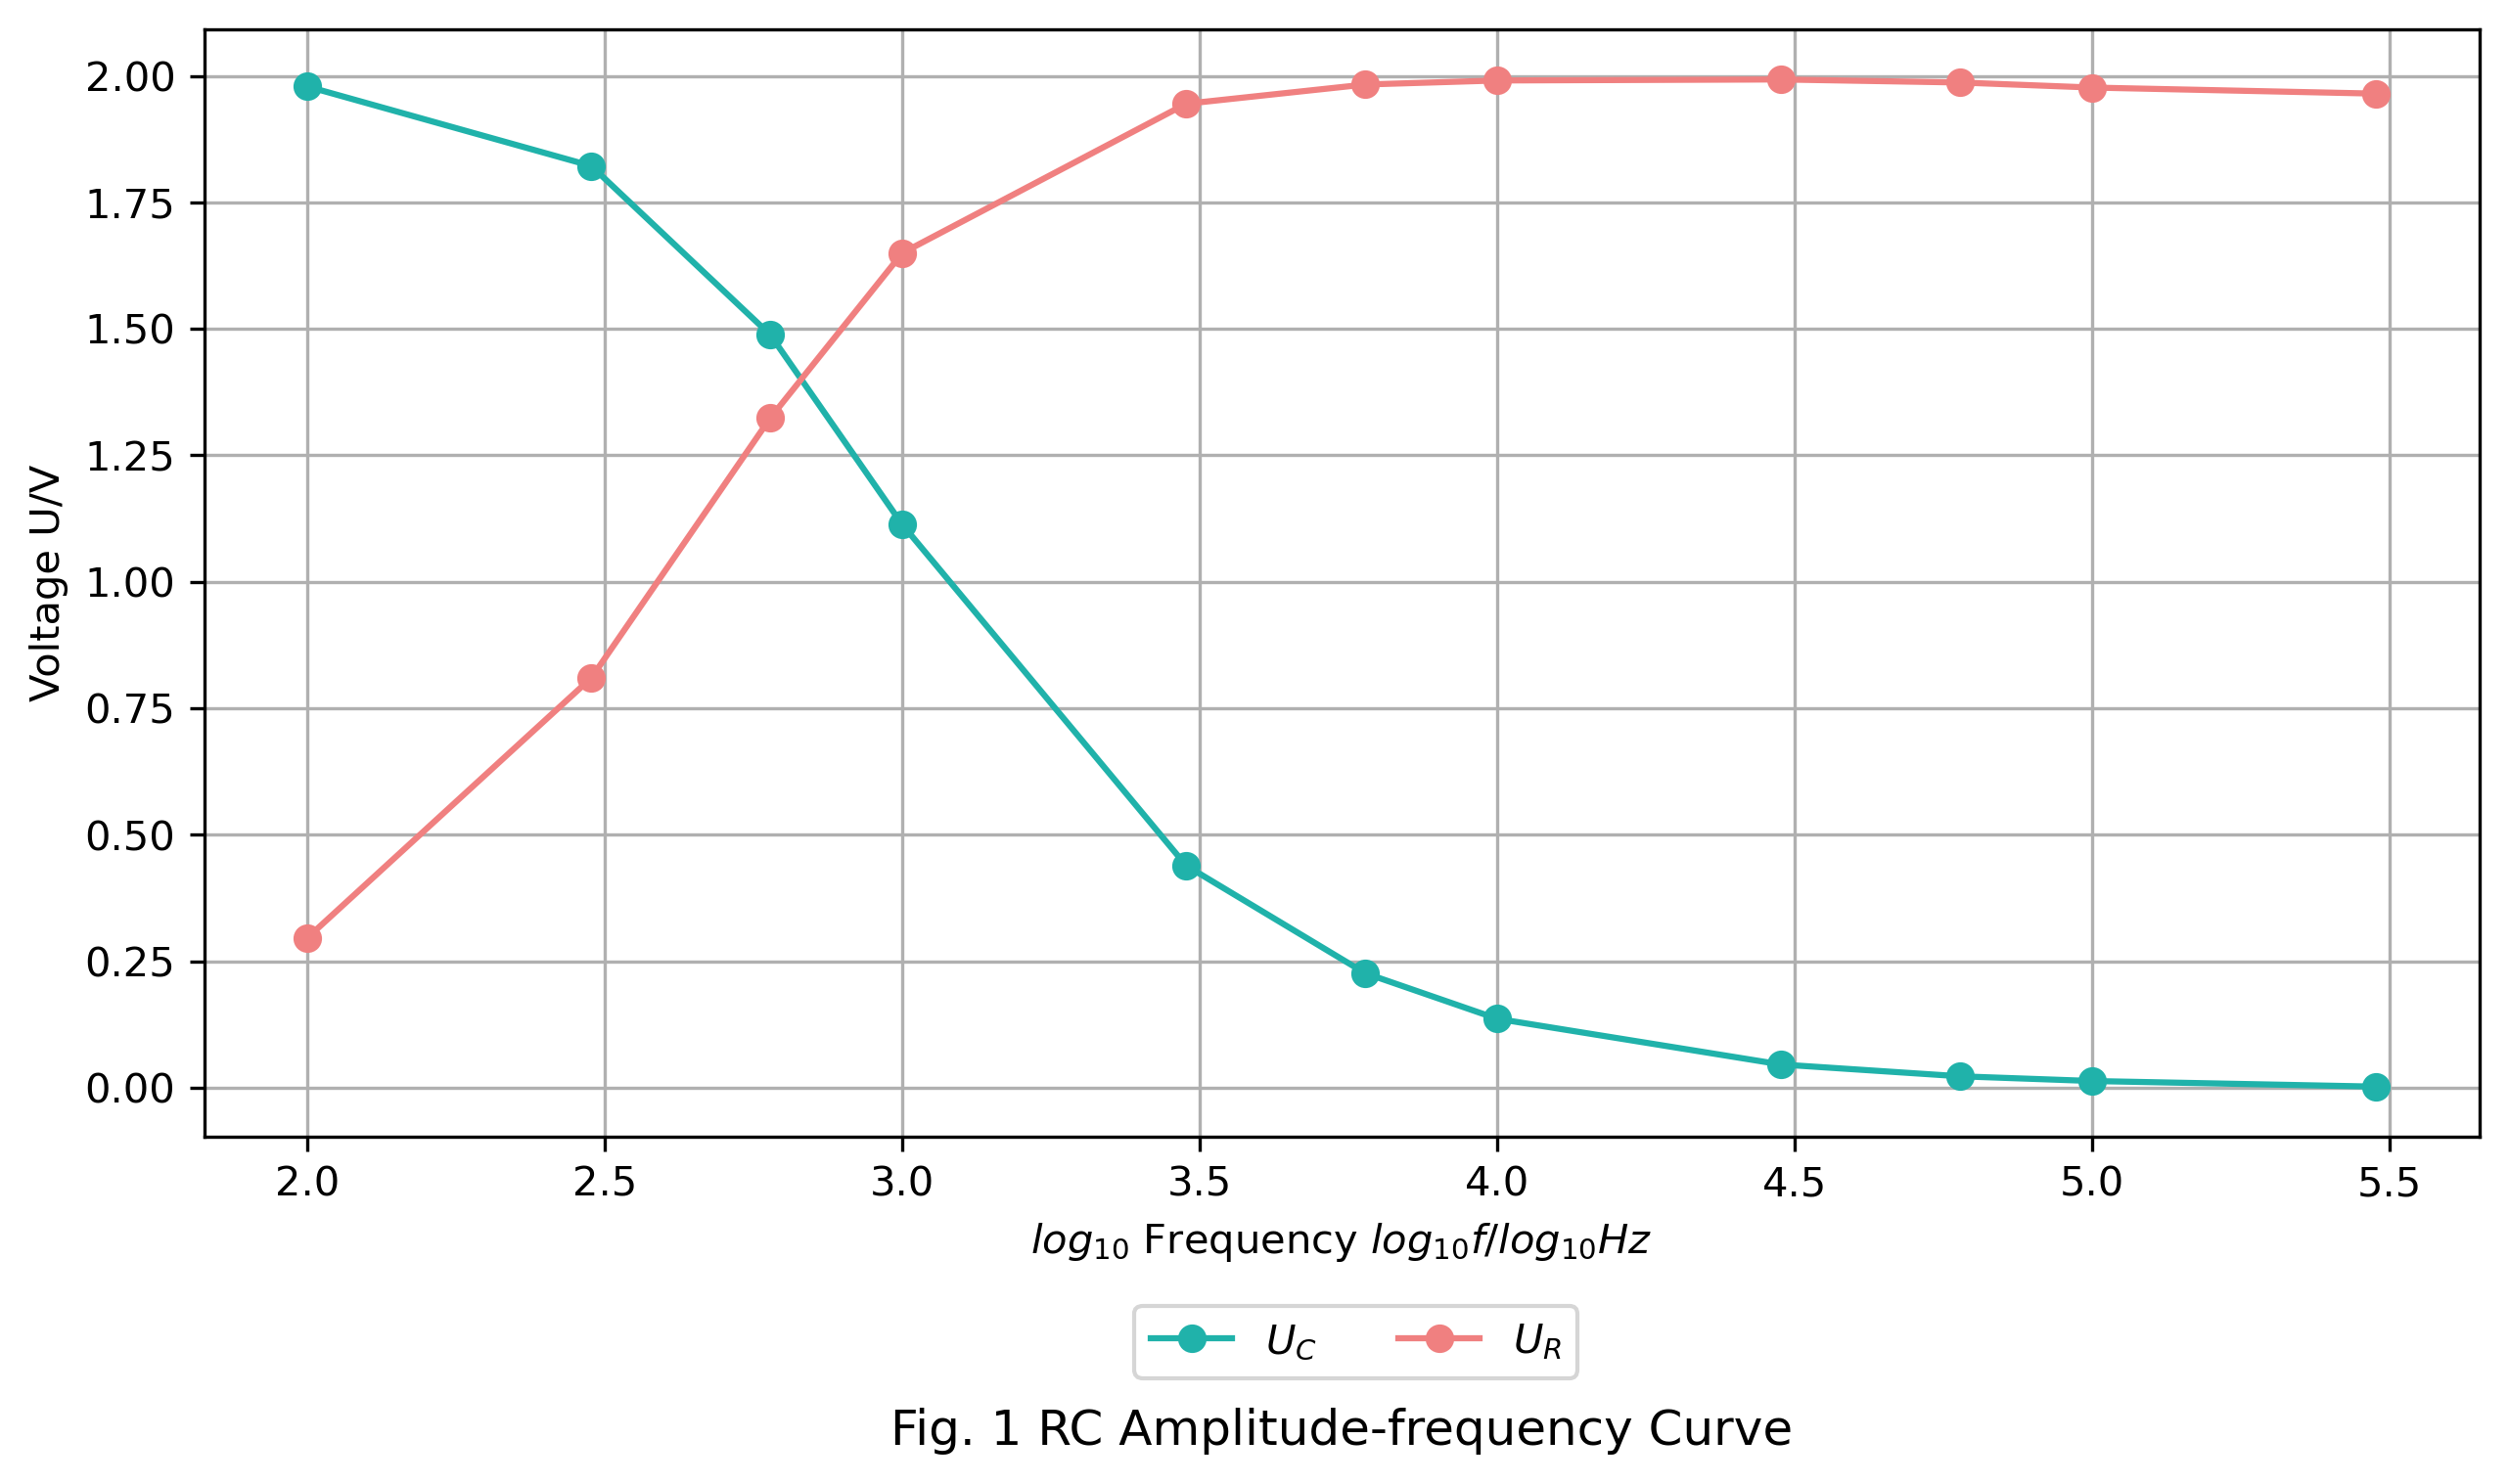
\includegraphics[width=0.23\textwidth]{attachments/fig.2.2.1.png}
				}
				\subfloat[实验相频曲线]{\label{fig:2.2.2}
				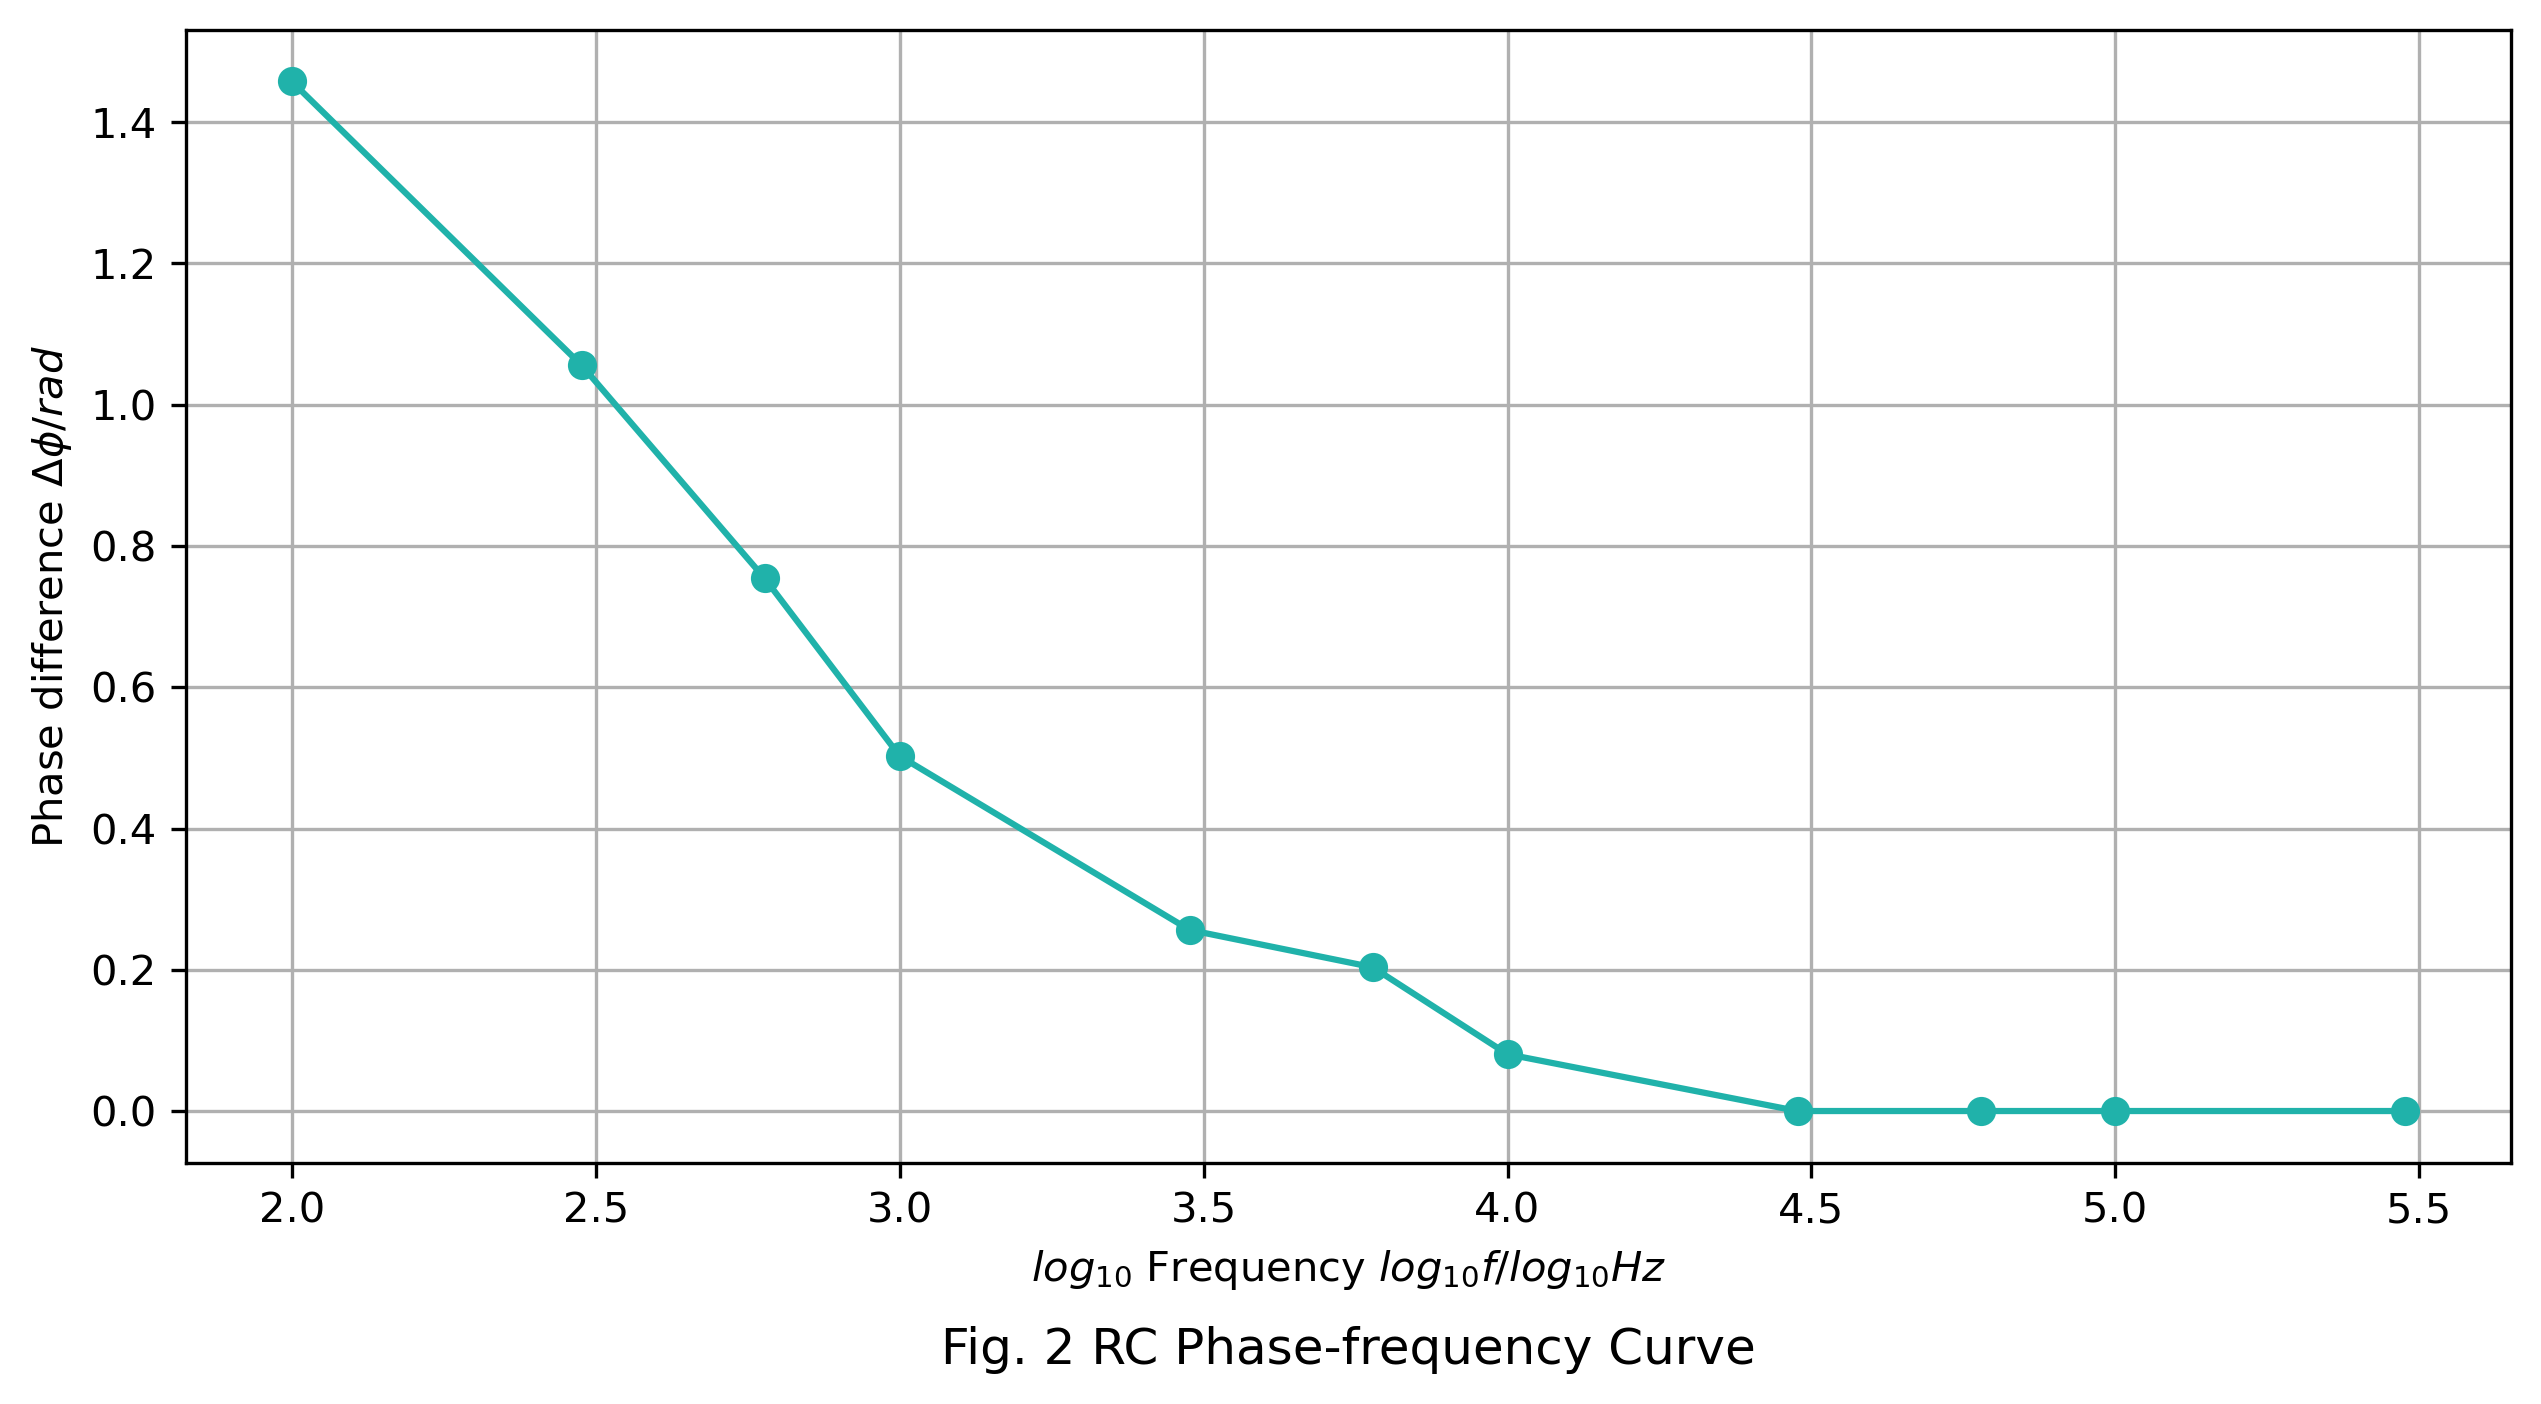
\includegraphics[width=0.23\textwidth]{attachments/fig.2.2.2.png}
				}
				\caption{RC电路}
			\end{figure}

			\paragraph{A. RL电路}~
			\newline 
			\indent
			RL电路仿真幅频曲线和相频曲线如图\ref{fig:2.3},对比B5实验结果,发现仿真与真实实验吻合。
			\begin{figure}[htbp]
				\centering
				\subfloat[RL仿真实验结果]{\label{fig:2.3}
				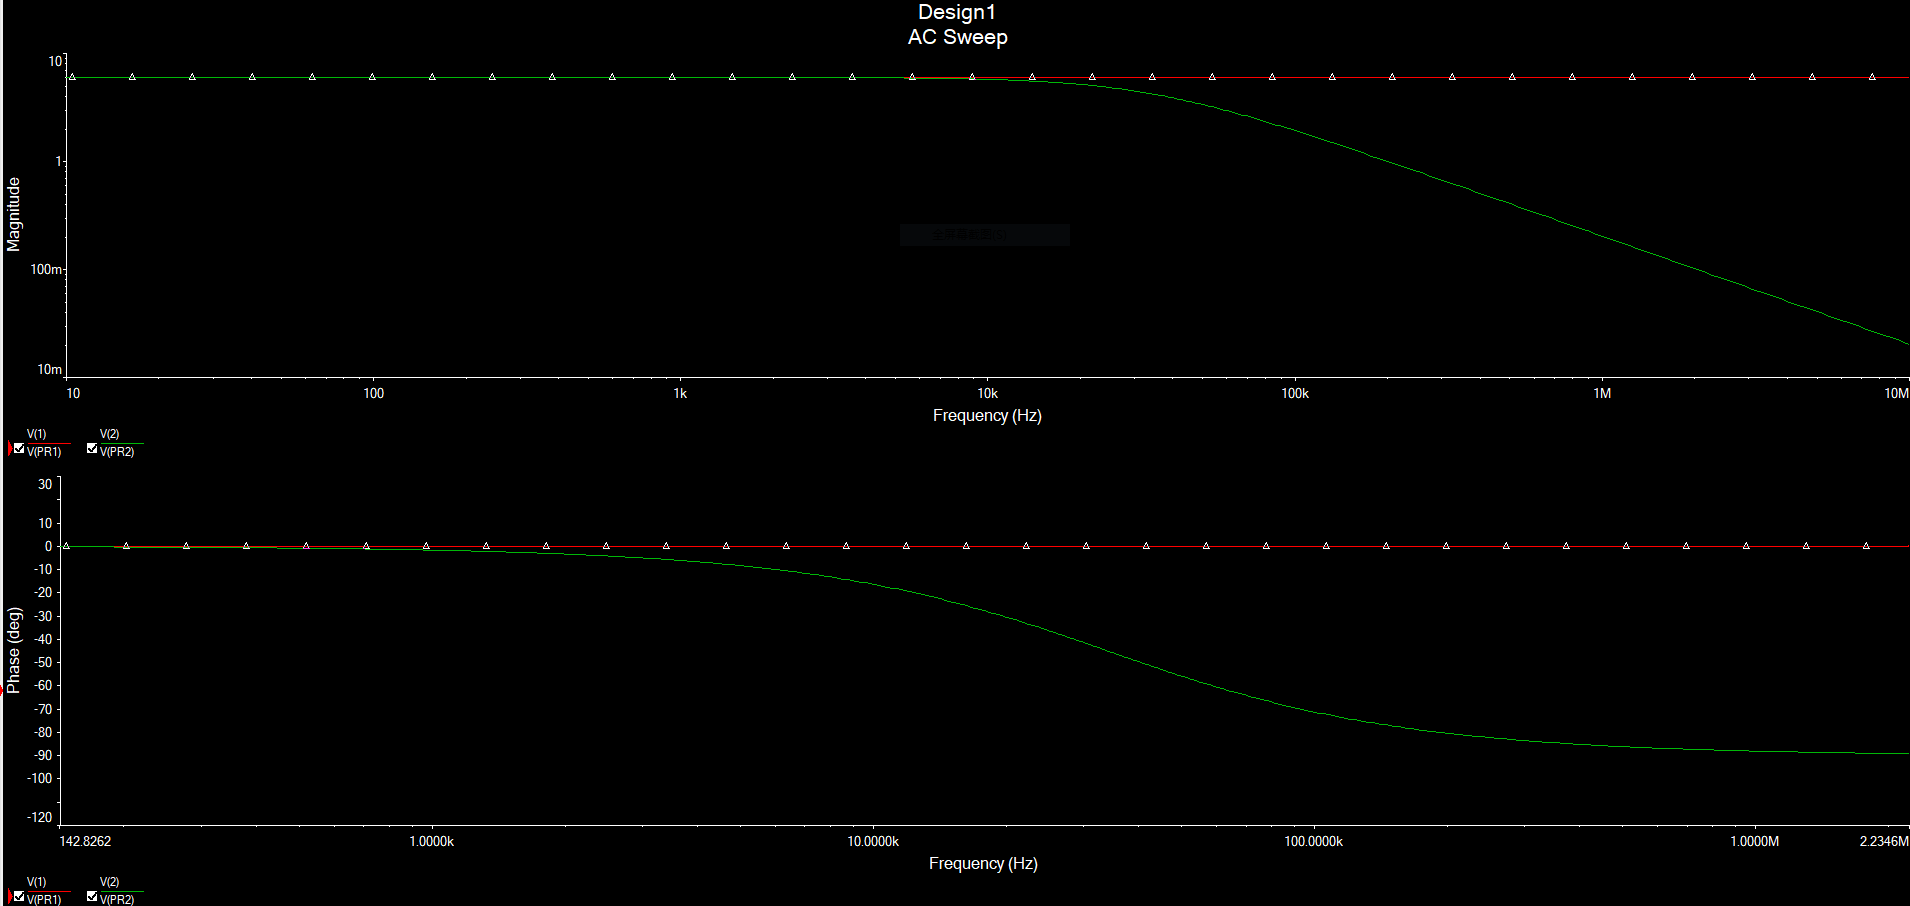
\includegraphics[width=0.3\textwidth]{attachments/fig.2.3.png}
				}		
				
				\subfloat[实验幅频曲线]{\label{fig:2.3.1}
				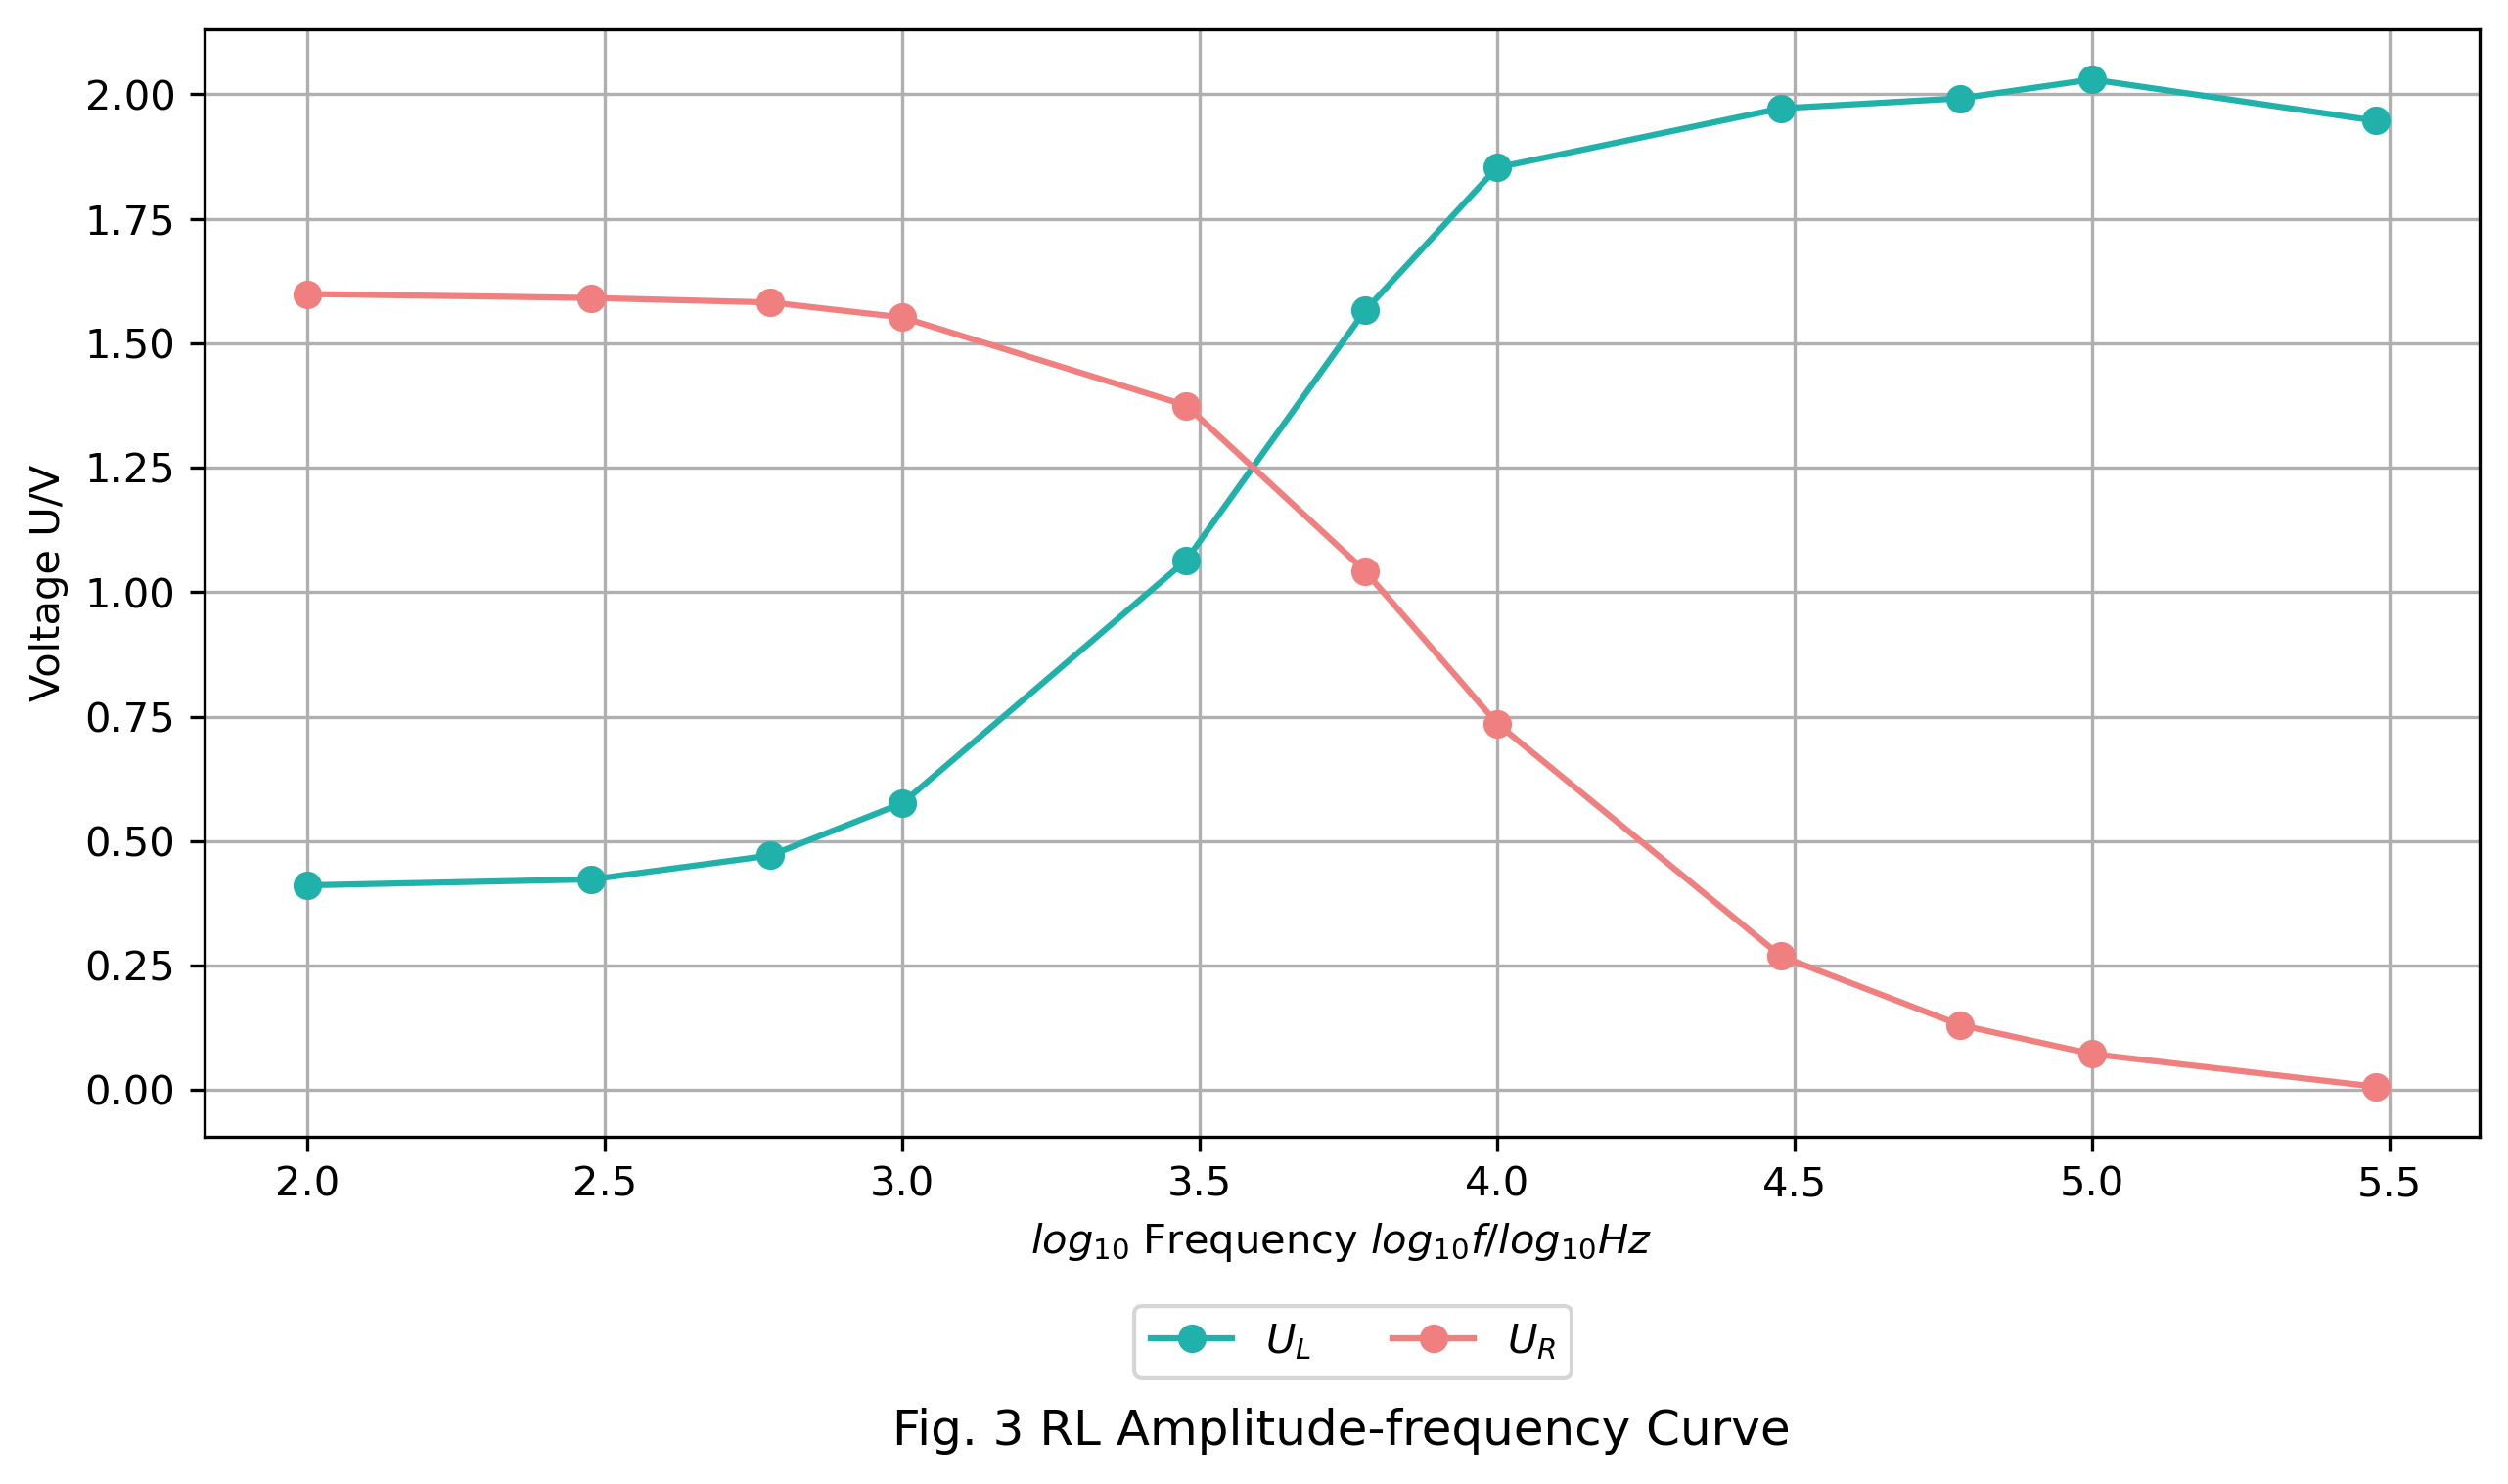
\includegraphics[width=0.23\textwidth]{attachments/fig.2.3.1.png}
				}
				\subfloat[实验相频曲线]{\label{fig:2.3.2}
				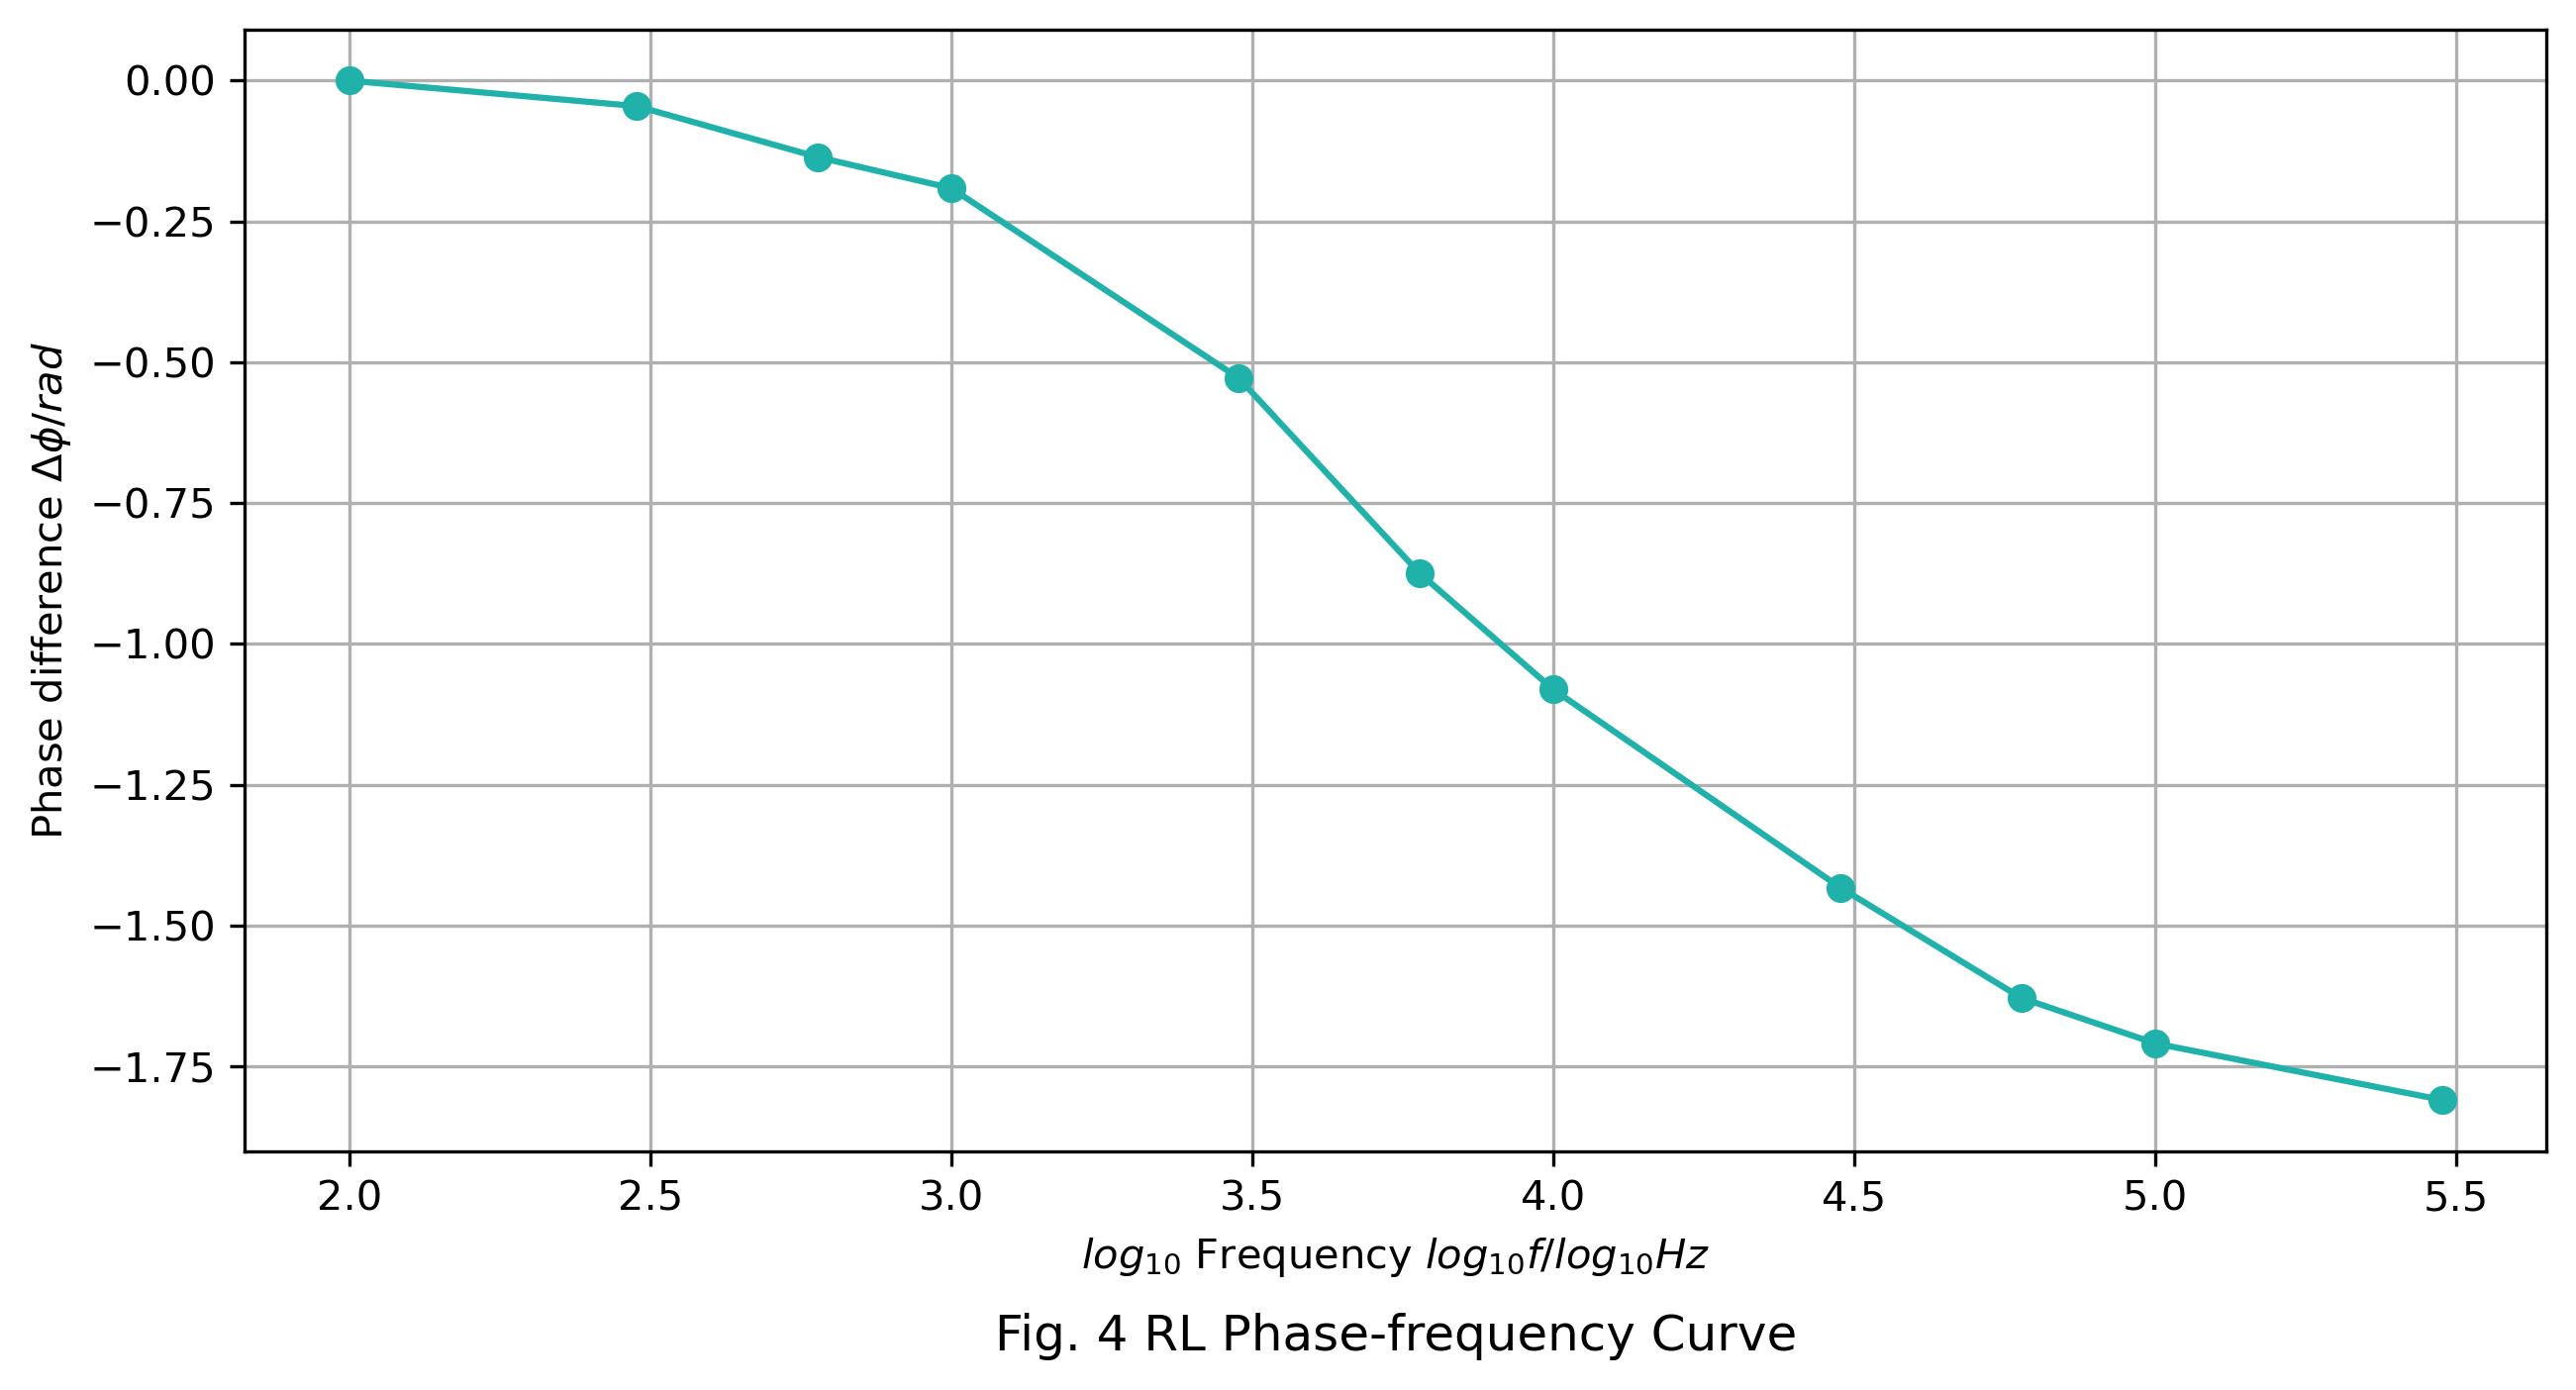
\includegraphics[width=0.23\textwidth]{attachments/fig.2.3.2.png}
				}
				\caption{RL电路}
			\end{figure}
		\subsubsection{非平衡直流电桥仿真实验}
			等变化$\Delta R$反向调节两电阻,$\Delta R$与电压表示数$U$关系如表\ref{tab:3}
			\begin{table}[htbp]
				\centering
					\begin{tabular}{cccccc}
						\toprule
						$\Delta R /Omega$	&0.00	&0.25	&0.50	&0.75	&1.00 	\\
						\midrule
						$U /mV$				&0 		&10		&20 	&30 	&40		\\
						\bottomrule
					\end{tabular}
					\caption{\textbf{非平衡直流电桥仿真实验}}
					\label{tab:3}
			\end{table}
			
			理论上,根据式\ref{eq:3},代入相关参数并略去二阶小量计算得
			$\Delta U = 0.04 \Delta R$,实验结果与理论相符。
	\subsection{黑箱实验}
		分别用万用表电阻档(表\ref{tab:4.1})、万用表电容档(表\ref{tab:4.2})
		和交流电桥(表\ref{tab:4.3})测量各接口间电路参数,结果如下
		\begin{table}[htbp]
			\centering
				\begin{tabular}{cccccc}
					\toprule
					1-2	&1-3	&1-4	&2-3	&2-4	&3-4 	\\
					\midrule
					$\infty$	&$\infty$ 	&$\infty$	&988.22$\Omega$ 	&0.3000$\Omega$ 	&988.19$\Omega$	\\
					\bottomrule
				\end{tabular}
				\caption{\textbf{万用表电阻档测量黑箱}}
				\label{tab:4.1}
		\end{table}
		\begin{table}[htbp]
			\centering
				\begin{tabular}{cccccc}
					\toprule
					1-2	&1-3	&1-4	&2-3	&2-4	&3-4 	\\
					\midrule
					69.8$nF$	&69.5$nF$ 		&69.8$nF$		&- 	&- 	&-		\\
					\bottomrule
				\end{tabular}
				\caption{\textbf{万用表电容档测量黑箱}}
				\label{tab:4.2}
		\end{table}
		\begin{table*}[htbp]
			\centering
				\begin{tabular}{ccccccc}
					\toprule
					参数	&1-2	&1-3	&1-4	&2-3	&2-4	&3-4 	\\
					\midrule
					$L /mH$	&-3.708 &-3.710	&-3.708	&2.49e-3 	&0.02e-3	&2.63e-3	\\
					$Q$	&0.2351 &93.538	&0.2351 &0.0002	&0.0829 &0.002	\\
					$C /nF$	&68.309 &68.260	&68.317	 &-106.9e+3	&-9024e+3	&-90.03e+3 \\
					$D$	&4.2534 &0.0107	&4.2539	 &6643.7	&12.180	&5592.0 \\
					\bottomrule
				\end{tabular}
				\caption{\textbf{交流电桥测量黑箱}}
				\label{tab:4.3}
		\end{table*}

		根据实验结果分析得黑箱电路结构如\ref{fig:3}。相关元件参数在图中标明。
		\begin{figure}[htbp]
			\centering
			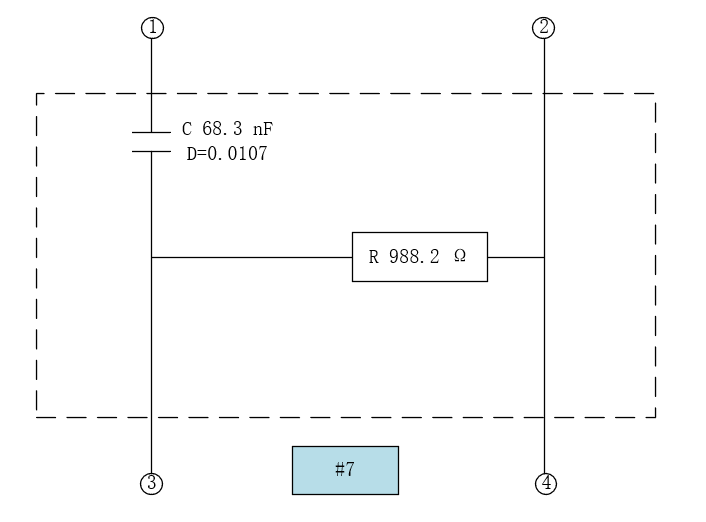
\includegraphics[width=0.4\textwidth]{attachments/fig.3.png}
			\caption{\#7黑箱电路结构}
			\label{fig:3}
		\end{figure}

\section{讨论}
	\subsection{电容、电感测量}
		对比手动调节电桥实验($exp$)结果、自动电桥($dig$)测量结果及仿真实验($sim$)结果,
		并计算自动电桥和仿真实验相对真实实验的百分偏差(exp\_dig和exp\_sim)。
		
		电容测量对比如表\ref{tab:5.1},电感测量对比如表\ref{tab:5.2}
		\begin{table}[htbp]
			\centering
				\begin{tabular}{ccccc}
					\toprule
					实验	&$C_x/ nF$	&$r_C/ \Omega$	&$Z_C/ \Omega$	&$D$ \\
					\midrule
					exp	&122.2	&43.3	&137.2	&0.332223	\\ 
					dig	&97.5	&52.5	&171.4	&0.322100	\\
					sim	&100.0	&51.0	&167.1	&0.320411	\\
					exp\_dig	&20.2\%	&21.3\%	&24.9\%	&3.0\%	\\
					exp\_sim	&18.2\%	&17.9\%	&21.8\%	&3.6\%	\\
					\bottomrule
				\end{tabular}
				\caption{\textbf{电容测量结果对比}}
				\label{tab:5.1}
		\end{table}
		\begin{table}[htbp]
			\centering
				\begin{tabular}{ccccc}
					\toprule
					实验	&$L_x/ \mH$	&$r_L/ \Omega$	&$Z_L/ \Omega$	&$Q$ \\
					\midrule
					exp	&19.8	&100.1	&1245.3	&12.4	\\
					dig	&19.9	&133.9	&1257.0	&9.3	\\
					sim	&20.0	&100.0	&1260.0	&12.6	\\
					exp\_dig	&0.7\%	&33.7\%	&0.9\%	&25.0\%	\\
					exp\_sim	&1.2\%	&0.08\%	&1.2\%	&1.3\%	\\
					\bottomrule
				\end{tabular}
				\caption{\textbf{电感测量结果对比}}
				\label{tab:5.2}
		\end{table}

		分析实验结果发现:电容测量实验中,除损耗因数D三个实验测量结果相近外,
		其余参量手动测量结果与数字电桥及仿真测量结果相差较大,相对误差均在20\%左右,而后两者测量结果相近;
		电感测量实验中,手动测量结果与仿真实验结果相近,相对误差均在1\%左右,而数字电桥测量结果与前两者相差较大。

		分析可能误差因素有:
		\begin{enumerate}[label=\arabic*.]
			\item 在实际电路实验中,不可能将电桥调节到完全平衡。事实上,由于电阻箱调节精度限制,我们只能将电压最低调至$1-5mV$量级,近似认为电桥平衡。
			\item 电桥两电阻阻值调节对电压差改变的影响程度是不同的,从而导致难以精确调配两电阻阻值。我们推测这也是电容实验偏差较大原因之一。
			\item 实际电路实验中使用面包板和导线连接电路,导线接头电阻及线路内阻会引入额外的电阻,从而导致桥臂电阻测量无法精确控制。
		\end{enumerate}

	\subsection{黑箱电路分析}
	已知限制条件:黑箱中仅可能有电阻、电容和电感元件;电路中至多有三个元件,每种元件至多只有一个;无并联电路。
	依据表\ref{tab:4.1},\ref{tab:4.2}和\ref{tab:4.3},分析如下:
	\begin{enumerate}[label=\arabic*.]
		\item 由表\ref{tab:4.1}:12、13、14间应为断路或有一电容;24间为短路或可能有电感;23、24间应有纯电阻,可能有电感。
		\item 由表\ref{tab:4.2}:确认12、13、14间有一电容,考虑限制条件,电容在1端口处。
		\item 由表\ref{tab:4.3}:由电感测量数据,证实24间为短路,23、34间有一微弱电感(2.5$\mu H$左右),推测为绕线电阻电感,证实了23、34间为纯电阻。
		\item 综合以上分析,绘制电路图如\ref{fig:3}
	\end{enumerate}

%%end-------------------正文-----------------------%%

%%end--------------------结论和引用------------------------%%
\section{结~~~论}
	本次实验中,我们搭建电感、电容交流电桥,手动调节电桥平衡,计算未知电感和未知电容阻值,并用自动电桥和仿真平台对结果进行了验证。
	我们发现手动测量需要细致调节电桥平衡,且受元件性能影响大,测量随机性大且不确定性高。
	而自动电桥能快速自动调节电桥平衡,稳定性好,结果精确。
	同时我们发现,预先借助电学仿真平台搭建仿真电路进行初步探索,有助于确定实际实验参数范围,提高实验效率。

\printbibliography[title=参考文献] 
%%end--------------------结论和引用------------------------%%


%%begin------------------英文摘要------------------------%%
\twocolumn[
\begin{@twocolumnfalse}
	\renewcommand{\abstractname} {} 
	\begin{center}
	    {\LARGE\bfseries Measured the unknown inductor and capacitor with AC bridge and simulation experiment on $Multisim$ platform \footnotemark[1]  \par}
	    \vskip 1.4em
	    {\large
	     \lineskip .75em
	      \begin{tabular}[t]{c}
	        \large Ziwei, Huang$^{1}$
	      \end{tabular}\footnotemark[2] \par
	      }
	      \vskip 0.4em
	    {\normalsize 1 Zhongshan School of Medicine, Sun Yat-sen University, Guangzhou  { \rm 510275}, China}
	\end{center}
	\begin{abstract}
		\vspace{-2em}  
	    	{\bf Abstract:}
	     {\small The AC bridge is a classic experimental circuit. Based on the bridge balance principle, AC bridge can be used to measure the parameters of unknown circuit components. 
         This measurement method is simple and convenient with high accuracy, and has wide applications in high-precision measurement, automatic control and other fields. 
         In this experiment, we measure the capacitance, impedance and loss factor of the unknown capacitor using capacitor bridge, and the inductance, impedance and quality factor of the unknown inductor using Maxwell-Vine bridge. 
         These results were compared with the results measured with digital bridge meter. 
         We also conducted simulation experiments on the $Multisim$ circuit simulation platform and compared them with the real experimental results to investigate the factors affecting the results of this experiment. 
         It was found that the capacitance measurement results differed from the digital bridge and simulation, and the latter two results were similar; while the inductance measurement results were similar to the simulation results, and the digital bridge measurement differed from the former two. 
         The key point of this experiment is the fineness of the adjustment of the AC bridge equilibrium state, and the biggest factor limiting the accuracy of the experiment is the precision of the experimental instrument.}
	  	\par
		\textbf{Key words}:AC bridge, capacitor, inductor, $Multisim$ simulation experiment
	\end{abstract}
\end{@twocolumnfalse}
]
\footnotetext[1]{{Supported and taught by Luyoutang, School of Physics, Sun Yat-sen University}}
\footnotetext[2]{{Corresponding author. \url{huangzw29@mail2.sysu.edu.cn}}}
%%end--------------------英文摘要------------------------%%
\end{document}